\clearpage

\refstepcounter{chapter}
\chapter*{Pruebas y Validaciones}

\addcontentsline{toc}{chapter}{\protect\numberline{\thechapter}Pruebas y Validaciones}
\vspace{-1.5cm}
\noindent\HRule\par\vspace{0.1cm}




\section{Planificación de las Pruebas}

La validación del sistema se organizó de forma progresiva, comenzando por los componentes más básicos y avanzando hasta pruebas completas de seguimiento. La idea principal fue no evaluar directamente el sistema completo, sino comprobar primero cada bloque por separado y, después, analizar si todos funcionan de forma coordinada dentro del lazo de seguimiento visual.

\vspace{0.3cm}

De forma esquemática, la planificación de las pruebas se estructuró del siguiente modo:

\begin{itemize}
    \item \textbf{Definición de métricas de evaluación.} Antes de ejecutar los experimentos se definen las magnitudes que permiten interpretar los resultados: precisión del detector, tiempo de inferencia, tamaño del modelo, error visual de centrado, error de distancia, tiempo de establecimiento y continuidad de la detección. Con ello se intenta demostrar que la comparación entre pruebas se apoya en criterios objetivos y no únicamente en una valoración visual.

    \item \textbf{Selección del detector YOLO.} Se comparan distintas versiones de YOLO bajo condiciones equivalentes, atendiendo al equilibrio entre precisión, velocidad y tamaño. Con esta prueba se intenta demostrar que el modelo elegido no solo detecta correctamente el UAV objetivo, sino que también puede integrarse en un sistema de control en tiempo real sin introducir una carga computacional excesiva.

    \item \textbf{Optimización del detector con TensorRT.} Tras seleccionar el modelo, se evalúa su conversión a TensorRT para el despliegue en una plataforma Jetson, comparando los tiempos de preprocesamiento, inferencia y postprocesamiento del modelo original y del modelo optimizado. Con esta prueba se intenta demostrar que la optimización reduce la latencia del detector y deja margen temporal para ejecutar el resto de nodos de ROS, MAVROS, filtrado y control.

    \item \textbf{Validación individual de los controladores PID.} Se evalúan por separado los controladores de \textit{yaw}, altura y distancia, de manera que la respuesta de cada eje pueda analizarse sin mezclar efectos de otros controladores. Con esta prueba se intenta demostrar que cada PID reduce su error asociado de forma estable y con un tiempo de respuesta aceptable.

    \item \textbf{Prueba conjunta de control visual.} Una vez validados los controladores por separado, se activan conjuntamente los tres PID para comprobar la respuesta global del UAV cazador. Con esta prueba se intenta demostrar que las salidas de los controladores son compatibles entre sí y que los errores visuales y de distancia pueden transformarse en consignas de movimiento coherentes.

    \item \textbf{Seguimiento en trayectorias simuladas.} En simulación se prueban trayectorias más completas, como movimientos en zigzag, trayectorias circulares con cambios de altura y una ruta final por \textit{waypoints}. Con estas pruebas se intenta demostrar que el sistema mantiene el seguimiento cuando el UAV objetivo se mueve de forma dinámica y aparecen variaciones de posición, escala y orientación.

    \item \textbf{Prueba con cámara real.} Finalmente, se realiza una primera validación con el UAV objetivo físico, centrada en la estimación de distancia a partir del tamaño aparente de la caja detectada. Con esta prueba se intenta demostrar que la percepción desarrollada en simulación puede trasladarse a imágenes reales y producir una estimación de distancia coherente en rangos cercanos y medios.
\end{itemize}

\vspace{0.3cm}

Esta planificación permite avanzar desde una validación aislada de cada módulo hasta una evaluación global del sistema. Así, los resultados de cada prueba no solo indican si un bloque funciona, sino también qué limitaciones puede introducir cuando se integra con el resto de la arquitectura.


\section{Desarrollo de los Experimentos}

\subsection{Métricas de Evaluación}

Para comparar las distintas pruebas de esta sección se emplearon métricas asociadas a cuatro aspectos del sistema: la calidad del detector visual, el rendimiento de inferencia, la respuesta de los controladores y la continuidad del seguimiento del objetivo. De este modo, no solo se analiza si el UAV objetivo se detecta correctamente, sino también si las señales generadas por la percepción son suficientemente estables para alimentar el lazo de control.

\vspace{0.3cm}


\begin{itemize}
    

    \item \textbf{Selección del detector YOLO.} En este experimento se comparan modelos de detección. Se utilizan el número de parámetros, el tiempo de inferencia, $\mathrm{mAP}_{50}$ y $\mathrm{mAP}_{50-95}$. El tiempo medio de inferencia se calcula como:
    \[
    t_{\mathrm{inf}}=\frac{1}{N}\sum_{i=1}^{N}t_i,
    \]
    donde $t_i$ es el tiempo necesario para procesar la imagen $i$ y $N$ es el número total de imágenes evaluadas. Esta métrica sirve para saber si el detector puede ejecutarse suficientemente rápido dentro del lazo de control. La precisión se mide mediante:
    \[
    \mathrm{mAP}_{50}=\frac{1}{C}\sum_{c=1}^{C}AP_c(0.50),
    \]
    \[
    \mathrm{mAP}_{50-95}=\frac{1}{10C}\sum_{\tau\in\{0.50,0.55,\ldots,0.95\}}\sum_{c=1}^{C}AP_c(\tau).
    \]
    En estas expresiones, $AP_c$ es el área bajo la curva precisión--recobrado de la clase $c$, $C$ es el número de clases y $\tau$ representa el umbral de \textit{IoU}. La métrica $\mathrm{mAP}_{50}$ indica la calidad general de detección, mientras que $\mathrm{mAP}_{50-95}$ es más exigente porque penaliza cajas delimitadoras peor ajustadas. El número de parámetros complementa estas métricas indicando el tamaño y coste computacional del modelo.

    \item \textbf{Optimización del detector con TensorRT.} En este experimento se evalúa si el detector seleccionado puede ejecutarse con menor latencia en la plataforma Jetson. Para ello se separa el tiempo total de procesamiento en tres partes:
    \[
    t_{\mathrm{total}}=t_{\mathrm{pre}}+t_{\mathrm{inf}}+t_{\mathrm{post}},
    \]
    donde $t_{\mathrm{pre}}$ es el tiempo de preprocesamiento, $t_{\mathrm{inf}}$ es el tiempo de inferencia y $t_{\mathrm{post}}$ es el tiempo de postprocesamiento. A partir del tiempo total se calcula la frecuencia máxima teórica:
    \[
    \mathrm{FPS}_{\mathrm{teor}}=\frac{1000}{t_{\mathrm{total}}},
    \]
    expresando $t_{\mathrm{total}}$ en milisegundos. Estas métricas sirven para comprobar si la conversión a TensorRT reduce la latencia y si queda margen temporal para ejecutar, además del detector, los nodos de ROS, MAVROS, filtrado y control.

    \item \textbf{Validación individual de los controladores PID.} En estas pruebas se evalúa cada eje de control por separado. Para el centrado visual se utilizan los errores normalizados:
    \[
    E_{x,i}=\frac{u_i-W/2}{W/2}, \qquad E_{y,i}=\frac{v_i-H/2}{H/2},
    \]
    donde $(u_i,v_i)$ es el centro de la caja detectada en el frame $i$, y $W$ y $H$ son la anchura y la altura de la imagen. El error $E_x$ sirve para evaluar el PID de \textit{yaw}, ya que mide el desplazamiento horizontal del objetivo. El error $E_y$ sirve para evaluar el PID de altura, ya que mide el desplazamiento vertical. Para el eje longitudinal se utiliza:
    \[
    E_{z,i}=d_i-d_{\mathrm{ref}},
    \]
    donde $d_i$ es la distancia estimada al objetivo y $d_{\mathrm{ref}}$ es la distancia deseada de seguimiento. Además, se calcula el tiempo de establecimiento:
    \[
    T_s=\min\{t_s: |e(t)|\leq\varepsilon,\; \forall t\geq t_s\}.
    \]
    Esta métrica indica cuánto tarda cada controlador en entrar y permanecer dentro de una banda de tolerancia $\varepsilon$. En conjunto, estas medidas permiten comprobar si cada PID reduce su error de forma estable antes de combinar los tres ejes.

    \item \textbf{Prueba conjunta de control visual.} En este experimento se activan simultáneamente los PID de \textit{yaw}, altura y distancia. Para resumir el error de centrado en imagen se utiliza el EPE 2D:
    \[
    \mathrm{EPE}_i=\sqrt{E_{x,i}^{2}+E_{y,i}^{2}}.
    \]
    Esta métrica combina el error horizontal y vertical en una única magnitud, por lo que sirve para saber si el objetivo se mantiene cerca del centro de la cámara. Para el eje longitudinal se utiliza el RMSE de distancia:
    \[
    \mathrm{RMSE}_{z}=\sqrt{\frac{1}{|\mathcal{I}_{\mathrm{V}}|}\sum_{i\in\mathcal{I}_{\mathrm{V}}}E_{z,i}^{2}}.
    \]
    El RMSE penaliza más los errores grandes que los pequeños y permite detectar desviaciones importantes respecto a la separación deseada. Junto con la evolución temporal de  $E_z$, esta métrica sirve para comprobar que el controlador actúa de forma compatible y sin oscilaciones crecientes.

    \item \textbf{Seguimiento en trayectorias simuladas.}\\ En estas pruebas se evalúa el lazo cerrado completo durante trayectorias dinámicas. La continuidad de la percepción se mide mediante:
    \[
    P_{\mathrm{YOLO}}=\frac{N_{\mathrm{YOLO}}}{N}\cdot100, \qquad P_{\mathrm{Kalman}}=\frac{N_{\mathrm{Kalman}}}{N}\cdot100,
    \]
    \[
    \mathrm{TLR}=\frac{N_{\mathrm{perdidos}}}{N}\cdot100.
    \]
    En estas expresiones, $N$ es el número total de frames, $N_{\mathrm{YOLO}}$ es el número de frames con detección directa, $N_{\mathrm{Kalman}}$ es el número de frames mantenidos por predicción y $N_{\mathrm{perdidos}}$ es el número de frames sin referencia válida. $P_{\mathrm{YOLO}}$ sirve para medir la disponibilidad del detector, $P_{\mathrm{Kalman}}$ indica cuánto apoyo requiere el filtro predictivo y TLR mide la tasa de pérdida completa del objetivo. Además, el error de centrado se resume por estado de percepción:
    \[
    \mathrm{EPE}_{\mathrm{YOLO}}=\frac{1}{|\mathcal{I}_{\mathrm{YOLO}}|}\sum_{i\in\mathcal{I}_{\mathrm{YOLO}}}\mathrm{EPE}_i,
    \]
    \[
    \mathrm{EPE}_{\mathrm{Kalman}}=\frac{1}{|\mathcal{I}_{\mathrm{Kalman}}|}\sum_{i\in\mathcal{I}_{\mathrm{Kalman}}}\mathrm{EPE}_i,
    \]
    \[
    \mathrm{EPE}_{\mathrm{total}}=\frac{1}{|\mathcal{I}_{\mathrm{V}}|}\sum_{i\in\mathcal{I}_{\mathrm{V}}}\mathrm{EPE}_i.
    \]
    Esta separación permite comprobar si el seguimiento se mantiene principalmente con detecciones directas o si depende de la predicción. Los frames sin referencia válida no se promedian en EPE ni en RMSE; si el código marca una medida con un valor como $-999.0$, dicho valor se interpreta como pérdida de percepción y se contabiliza mediante el TLR.

    \item \textbf{Prueba con cámara real.} En este experimento se evalúa la estimación de distancia con imágenes reales. Para cada medida se calcula el error de distancia:
    \[
    e_{d,i}=\hat{d}_i-d^{\mathrm{real}}_i,
    \]
    donde $\hat{d}_i$ es la distancia estimada a partir de la caja detectada y $d^{\mathrm{real}}_i$ es la distancia medida físicamente. El error absoluto se define como:
    \[
    |e_{d,i}|=|\hat{d}_i-d^{\mathrm{real}}_i|,
    \]
    y resume cuánto se desvía la estimación en cada muestra sin tener en cuenta el signo. Para resumir el comportamiento global se utiliza el error medio absoluto:
    \[
    \mathrm{MAE}=\frac{1}{N}\sum_{i=1}^{N}|e_{d,i}|,
    \]
    y la desviación típica:
    \[
    \sigma_d=\sqrt{\frac{1}{N-1}\sum_{i=1}^{N}(e_{d,i}-\bar{e}_d)^2}.
    \]
    El MAE sirve para cuantificar el error medio de estimación, mientras que $\sigma_d$ indica la dispersión entre repeticiones. Analizar estas métricas en función de la distancia real permite identificar en qué rango la estimación es más fiable y a partir de qué separación comienza a degradarse.
\end{itemize}

\vspace{0.3cm}

\subsection{Selección del Modelo}

El primer experimento tuvo como objetivo seleccionar el detector más adecuado para el sistema de seguimiento visual. Para ello se realizó un torneo comparativo entre distintas arquitecturas de la familia YOLO, utilizando el dataset descrito previamente y manteniendo las mismas condiciones de entrenamiento para todos los modelos. El experimento se ejecutó en Google Colab, utilizando una GPU Nvidia T4 para entrenar de forma secuencial las variantes YOLOv8, YOLOv10, YOLO11 y YOLO26 en sus versiones \textit{nano} (n), \textit{small} (s) y \textit{medium} (m).

\vspace{0.3cm}

La comparación se planteó como un proceso automatizado en el que se recorría una lista de pesos preentrenados. Para cada arquitectura se cargaba el modelo correspondiente, se inicializaba a partir de sus pesos base y se realizaba un ajuste fino sobre el dataset del proyecto. De esta forma, todos los modelos partían de conocimiento visual previo y se especializaban posteriormente en la detección del UAV objetivo, siguiendo el mismo enfoque de \textit{fine-tuning} empleado para YOLOv8n en el capítulo de implementación.

\vspace{0.3cm}

Todos los entrenamientos se realizaron con una configuración común: 25 épocas, tamaño de imagen de $640 \times 640$ píxeles y \textit{batch size} de 16. Además, se mantuvo la selección automática del optimizador mediante \texttt{optimizer=auto}, de forma que Ultralytics determinara los hiperparámetros más adecuados para cada caso. Cada ejecución se guardó en un directorio independiente, identificado con el nombre del modelo entrenado, lo que permitió comparar posteriormente las métricas obtenidas de forma ordenada y homogénea.

\vspace{0.3cm}

Los resultados del torneo se resumen en la Tabla \ref{tab:comparativa-yolo}. Para la comparación se utilizaron cuatro criterios principales: número de parámetros, \textit{mAP50}, \textit{mAP50-95} y tiempo de inferencia. Estos indicadores permiten evaluar no solo la precisión del detector, sino también su coste computacional y su idoneidad para integrarse en un lazo de control en tiempo real.

\begin{table}[htbp]
\centering
\caption{Comparativa de modelos YOLO evaluados para la detección visual.}
\label{tab:comparativa-yolo}
\scriptsize
\setlength{\tabcolsep}{4pt}
\resizebox{\textwidth}{!}{%
\begin{tabular}{lcccc}
\hline
\textbf{Modelo} & \textbf{Parámetros (M)} & \textbf{mAP50} & \textbf{mAP50-95} & \textbf{Inferencia (ms)} \\
\hline
\textbf{YOLOv8n}  & \textbf{3.2}          & \textbf{0.992507} & \textbf{0.733692} & \textbf{2.660333}  \\
YOLOv8s  & 11.2         & 0.993716 & 0.734467 & 6.248403  \\
YOLOv8m  & 25.9         & 0.993991 & 0.750974 & 14.657198 \\
YOLOv10n & 2.3          & 0.988186 & 0.711153 & 3.258539  \\
YOLOv10s & 7.2          & 0.989443 & 0.726444 & 6.054465  \\
YOLOv10m & 16.4         & 0.983691 & 0.718956 & 14.397108 \\
YOLO11n  & 2.6          & 0.993189 & 0.728236 & 2.814279  \\
YOLO11s  & 9.4          & 0.994793 & 0.739400 & 6.217230  \\
YOLO11m  & 20.1         & 0.990841 & 0.716693 & 17.582637 \\
YOLO26n  & 2.4          & 0.986090 & 0.717900 & 2.899324  \\
YOLO26s  & 9.5          & 0.991955 & 0.732011 & 6.551616  \\
YOLO26m  & 20.04        & 0.988004 & 0.729559 & 17.643815 \\
\hline
\end{tabular}%
}
\end{table}

\vspace{0.3cm}

A partir de estos resultados se seleccionó YOLOv8n como modelo principal para el sistema de percepción. La elección no se basó únicamente en obtener el mayor valor de precisión absoluta, sino en encontrar el mejor compromiso entre precisión, velocidad de inferencia y tamaño del modelo. Este criterio es especialmente relevante en un sistema de seguimiento visual para UAV, donde el detector no trabaja de forma aislada, sino como parte de un lazo cerrado que debe proporcionar medidas frecuentes al controlador.

\vspace{0.3cm}

Desde el punto de vista de la precisión, YOLOv8n obtuvo un \textit{mAP50} de 0.992507 y un \textit{mAP50-95} de 0.733692, valores suficientemente altos para detectar el UAV objetivo de forma fiable. Aunque YOLOv8m alcanzó el mayor \textit{mAP50-95} de la tabla, con 0.750974, esta mejora fue reducida frente al incremento de coste computacional: YOLOv8m utiliza 25.9 millones de parámetros y requiere 14.657198 ms de inferencia, frente a los 3.2 millones de parámetros y 2.660333 ms de YOLOv8n. Por tanto, la ganancia de precisión no compensaba el aumento de tamaño ni el retardo introducido.

\vspace{0.3cm}

La comparación con YOLOv8s refuerza esta decisión, obteniendo un \textit{mAP50-95} muy similar, de 0.734467, pero aumentó el número de parámetros hasta 11.2 millones y el tiempo de inferencia hasta 6.248403 ms. Es decir, la mejora en precisión fue prácticamente despreciable para el objetivo del proyecto, mientras que el coste computacional creció de forma considerable. En un sistema de control visual, este incremento puede traducirse en menor frecuencia de actualización, mayor retardo en las correcciones y peor capacidad de reacción ante movimientos rápidos del UAV objetivo.

\vspace{0.3cm}

El resto de familias tampoco ofreció un compromiso superior. YOLOv10n y YOLO26n presentan menos parámetros que YOLOv8n, pero obtienen peores métricas de precisión y tiempos de inferencia superiores. YOLO11n mantiene un tamaño reducido y un \textit{mAP50} elevado, pero su \textit{mAP50-95} queda por debajo del de YOLOv8n y su inferencia también es ligeramente más lenta. Las variantes \textit{small} y \textit{medium} de YOLOv10, YOLO11 y YOLO26 incrementan el número de parámetros y el tiempo de inferencia sin aportar una mejora global suficiente para justificar su uso.

\vspace{0.3cm}

Por todo ello, YOLOv8n fue considerado el modelo más adecuado para el sistema implementado. Su principal ventaja es que mantiene una precisión elevada con el menor tiempo de inferencia de todos los modelos evaluados. Esta combinación permite alimentar al controlador con detecciones rápidas y suficientemente estables, reduciendo el riesgo de respuestas tardías, oscilaciones o pérdida temporal del objetivo durante las maniobras de seguimiento.

\subsection{Optimización del Modelo en Dron Real con TensorRT}

La selección de un detector ligero no es suficiente por sí sola cuando el sistema debe ejecutarse en un dron real. En este proyecto, el modelo de percepción está pensado para funcionar dentro de un sistema embarcado basado en una Jetson Origin Nano, donde los recursos de cómputo, memoria y consumo energético son más limitados que en un ordenador de sobremesa. Además, la detección no se utiliza de forma aislada: cada imagen procesada debe alimentar al filtro de Kalman y a los controladores PID del lazo IBVS, por lo que la inferencia debe realizarse con una latencia baja y de forma sostenida en el tiempo.

\vspace{0.3cm}

En este contexto, optimizar el modelo resulta necesario para que el detector pueda trabajar en tiempo real junto con el resto de nodos del sistema. Si la red neuronal introduce demasiado retardo, las medidas visuales llegan tarde al controlador y la respuesta del UAV cazador puede volverse menos precisa, especialmente cuando el objetivo realiza maniobras rápidas. Por este motivo, tras seleccionar YOLOv8n como detector principal, se evaluó su conversión a TensorRT, una herramienta orientada a acelerar la inferencia de redes neuronales en plataformas NVIDIA.

\vspace{0.3cm}

El experimento consistió en comparar el rendimiento del modelo original entrenado, almacenado en formato \texttt{.pt}, frente al mismo modelo exportado como motor TensorRT en formato \texttt{.engine}. La conversión no modifica el entrenamiento ni cambia la arquitectura utilizada para detectar el UAV, sino que transforma la red a una representación más eficiente para la GPU de la Jetson. Para ello se utilizó precisión reducida FP16, manteniendo el tamaño de entrada de $640$ píxeles:

\begin{lstlisting}[frame=none, numbers=none, backgroundcolor=\color{white}]
yolo export \
    model=~/catkin_ws/src/drone_lap/models/best.pt \
    format=engine \
    half=True \
    device=0 \
    workspace=2 \
    imgsz=640
\end{lstlisting}

\vspace{0.3cm}

La comparativa de rendimiento se realizó sobre 100 fotogramas con resolución de entrada $640 \times 480$ píxeles. En cada ejecución se midieron por separado los tiempos de preprocesamiento, inferencia en GPU y postprocesamiento, además del tiempo total medio por frame y los FPS máximos teóricos. Esta separación permite identificar si la mejora procede realmente de la ejecución de la red neuronal o de otras etapas del flujo de percepción. Los resultados se resumen en la Tabla \ref{tab:tensorrt-rendimiento}.

\begin{table}[H]
\centering
\caption{Comparativa de rendimiento antes y después de la optimización con TensorRT.}
\label{tab:tensorrt-rendimiento}
\begingroup
\footnotesize
\renewcommand{\arraystretch}{1.18}
\setlength{\tabcolsep}{6pt}
\resizebox{\textwidth}{!}{%
\begin{tabular}{lccccc}
\hline
\textbf{Ejecución} & \textbf{Preproc.} & \textbf{Infer. GPU} & \textbf{Postproc.} & \textbf{Total} & \textbf{FPS} \\
 & \textbf{(ms)} & \textbf{(ms)} & \textbf{(ms)} & \textbf{(ms/frame)} & \textbf{teóricos} \\
\hline
Modelo original \texttt{.pt} & 2.04 & 17.11 & 3.37 & 22.53 & 44.4 \\
TensorRT \texttt{.engine} FP16 & 2.26 & 5.75 & 3.73 & 11.74 & 85.2 \\
\hline
\end{tabular}%
}
\endgroup
\end{table}

\vspace{0.3cm}

La mejora principal se observa en la fase de inferencia. El tiempo de GPU pasó de $17.11\,\mathrm{ms}$ a $5.75\,\mathrm{ms}$, lo que supone una reducción aproximada del $66.4\%$. Esta diferencia se debe a que TensorRT genera un motor adaptado a la GPU concreta, selecciona operaciones más eficientes y aprovecha la precisión FP16. En la práctica, esto permite ejecutar la misma red neuronal con menor tiempo de cómputo, liberando recursos para el resto del sistema embarcado.

\vspace{0.3cm}

El tiempo total por fotograma se redujo de $22.53\,\mathrm{ms}$ a $11.74\,\mathrm{ms}$, una disminución cercana al $47.9\%$. En un sistema IBVS, este dato es especialmente importante porque el retardo entre la captura de la imagen y la reacción del UAV afecta directamente a la estabilidad del lazo de control. Al reducir la latencia, las medidas visuales que llegan al filtro de Kalman y a los controladores PID representan mejor el estado actual del objetivo, disminuyendo el riesgo de correcciones tardías cuando el UAV objetivo realiza maniobras rápidas.

\vspace{0.3cm}

También se aprecia un cambio en el cuello de botella del sistema. En la ejecución original, la inferencia en GPU representaba aproximadamente el $75.9\%$ del tiempo total, por lo que la red neuronal era el componente dominante. Tras la conversión a TensorRT, la inferencia baja hasta el $49.0\%$ del tiempo total y el conjunto de preprocesamiento y postprocesamiento pasa a tener un peso similar. Esto indica que la optimización ha desplazado la limitación principal desde la red neuronal hacia etapas auxiliares, ejecutadas principalmente mediante operaciones clásicas de tratamiento de imagen y preparación de datos.

\vspace{0.3cm}

La cámara utilizada trabaja a 30 FPS, por lo que cada imagen llega aproximadamente cada $33.3\,\mathrm{ms}$. Con el modelo original, el procesamiento consumía alrededor del $67.7\%$ de esa ventana temporal. Con TensorRT, el consumo baja hasta aproximadamente el $35.3\%$. Aunque la cámara no permite aprovechar directamente los $85.2$ FPS teóricos, este margen adicional resulta muy valioso: reduce la probabilidad de acumulación de retardos, facilita la ejecución concurrente de ROS, MAVROS y los controladores, y deja capacidad disponible para registrar datos, aplicar filtros o incorporar tareas adicionales sin saturar la Jetson.

\vspace{0.3cm}

En consecuencia, la conversión a TensorRT no solo aumenta la velocidad máxima teórica, que pasa de $44.4$ a $85.2$ FPS, sino que mejora la robustez temporal del sistema completo. El detector queda preparado para sensores de mayor frecuencia en trabajos futuros, pero incluso con una cámara de 30 FPS aporta beneficios directos: menor latencia, mayor margen de seguridad computacional, menor carga de GPU y una integración más adecuada para ejecución embarcada durante pruebas reales.

\subsection{Pruebas de Control}

\subsubsection{Pruebas Individuales en Simulación}

Estas pruebas sirven para comprobar por separado los tres controladores principales del sistema: \textit{yaw}, altura y distancia. Antes de activar el seguimiento completo, es necesario verificar que cada eje reduce su propio error de forma estable y que ninguna respuesta individual introduce oscilaciones o maniobras bruscas.

\vspace{0.3cm}

Con este bloque se responde a la pregunta de si cada PID es válido como componente aislado del lazo de control visual. Para ello, cada experimento excita principalmente un único eje mediante una trayectoria específica, se registra la evolución del error asociado y, después, se interpretan los resultados antes de combinar los tres controladores en una prueba conjunta.

\paragraph{Prueba del PID de \textit{yaw} con trayectoria circular}\mbox{}\par

Esta prueba sirve para validar el PID de \textit{yaw}, responsable de corregir el desplazamiento horizontal del objetivo en la imagen. La pregunta que se busca responder es si el UAV cazador puede girar de forma continua y estable para mantener al UAV objetivo cerca del centro horizontal de la cámara cuando este se desplaza lateralmente alrededor de él.

\vspace{0.3cm}

El experimento consiste en mantener el UAV cazador en una posición central mientras el UAV objetivo describe una trayectoria circular a su alrededor con un radio de 4 metros. Esta configuración genera un error horizontal variable y obliga al controlador a transformar dicho error visual en una consigna de giro de \textit{yaw}.

\vspace{0.3cm}

La trayectoria circular se generó actualizando de forma periódica la posición del UAV objetivo en el plano horizontal. Para ello, se calculó una velocidad angular a partir de la relación entre la velocidad lineal deseada y el radio de la circunferencia. Con un periodo de actualización de 20 Hz, en cada iteración se incrementó el tiempo de simulación, se obtuvo el ángulo instantáneo de la trayectoria y se calcularon las coordenadas del objetivo mediante las funciones trigonométricas seno y coseno. La altura se mantuvo constante durante toda la prueba, de modo que la variación principal observada por la cámara correspondiera al desplazamiento horizontal del objetivo.

\begin{figure}[H]
\centering
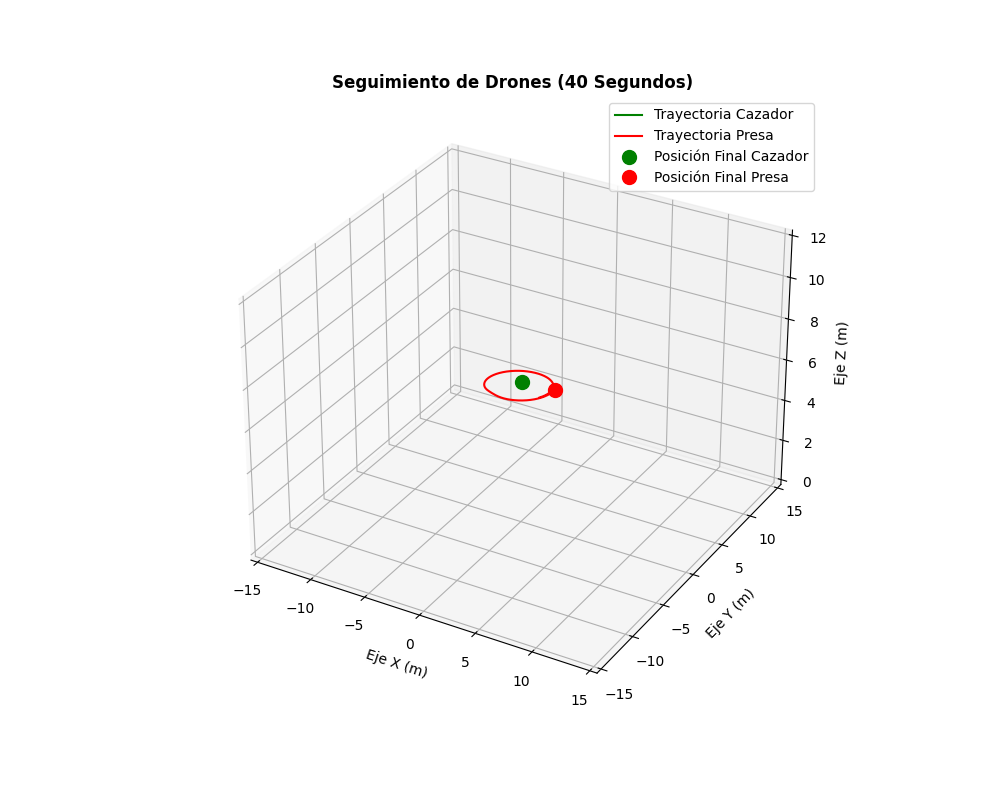
\includegraphics[width=1.0\textwidth]{imagenes/trayectoria3D-circular.png}
\caption{Trayectoria circular utilizada para la prueba del PID de \textit{yaw}. (Imagen de Elaboración Propia)}
\label{fig:trayectoria-circular-yaw}
\end{figure}

\vspace{0.3cm}

Como se observa en la Figura \ref{fig:trayectoria-circular-yaw}, el UAV objetivo realiza una circunferencia alrededor del UAV cazador, manteniendo una altura constante. Esta trayectoria resulta adecuada para analizar el control de \textit{yaw}, ya que obliga al sistema a corregir continuamente el error horizontal sin introducir cambios relevantes en el eje vertical.

\vspace{0.3cm}

La respuesta obtenida por el controlador se muestra en la Figura \ref{fig:respuesta-pid-yaw-circular}. La señal representada corresponde al error angular horizontal, denominado \texttt{Ex}, mientras que la línea discontinua roja indica la referencia deseada, es decir, error nulo. Al inicio de la prueba aparece un error negativo debido a que el objetivo no se encuentra perfectamente centrado en la imagen. Sin embargo, el PID corrige rápidamente esta desviación y lleva la señal hacia valores próximos a cero.

\begin{figure}[H]
\centering
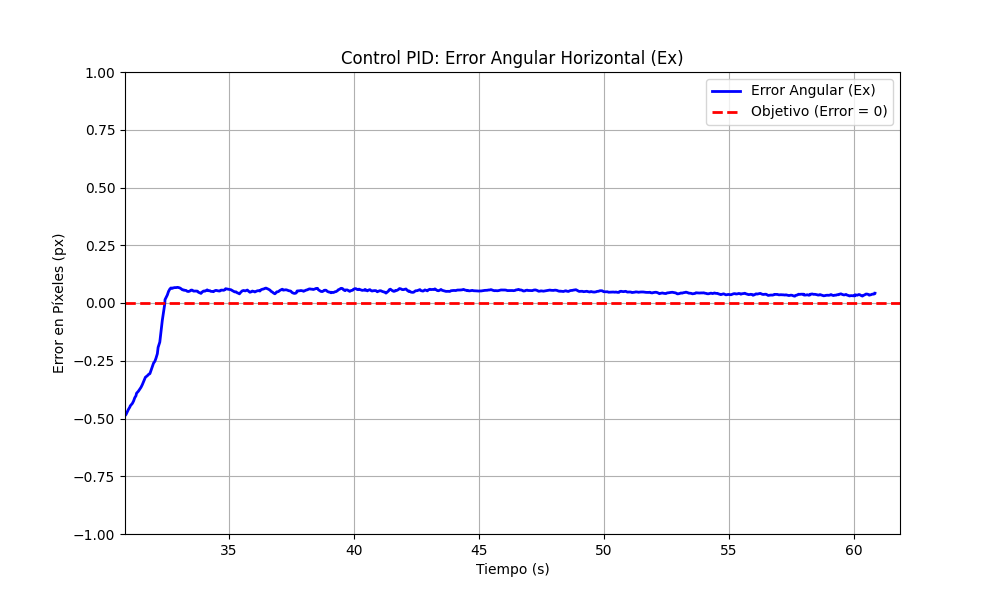
\includegraphics[width=0.95\textwidth]{imagenes/RespuestaPID_YAW_Circular.png}
\caption{Respuesta del PID de \textit{yaw} durante la trayectoria circular. (Imagen de Elaboración Propia)}
\label{fig:respuesta-pid-yaw-circular}
\end{figure}

\vspace{0.3cm}

La evolución de la señal muestra una respuesta estable tras el transitorio inicial. Aunque se aprecia un pequeño error residual positivo, este permanece acotado y con oscilaciones reducidas, lo que indica que el controlador mantiene el objetivo cerca del centro horizontal de la imagen durante la trayectoria circular. Por tanto, esta prueba confirma que el PID de \textit{yaw} es capaz de compensar el movimiento lateral relativo del UAV objetivo y generar una respuesta suficientemente suave para el seguimiento visual.

\paragraph{Prueba del PID de altura con trayectoria vertical}\mbox{}\par

Esta prueba sirve para validar el PID de altura, encargado de corregir el desplazamiento vertical del objetivo dentro de la imagen. Con ella se responde a la pregunta de si el UAV cazador puede modificar su altura de forma suave para mantener centrado al objetivo cuando este sube y baja durante el vuelo.

\vspace{0.3cm}

El experimento consiste en situar el UAV objetivo alrededor de una altura de referencia de 7 metros y hacerlo oscilar verticalmente alrededor de dicha posición. De esta manera se genera un error vertical controlado, sin introducir cambios dominantes en el eje horizontal, y se puede analizar la respuesta específica del controlador de altura.

\vspace{0.3cm}

La trayectoria se generó mediante una oscilación sinusoidal aplicada únicamente sobre la coordenada vertical del UAV objetivo. Para ello, se definió un valor central de altura, una amplitud de oscilación y un periodo de movimiento. En cada iteración, con una frecuencia de actualización de 20 Hz, se incrementó el tiempo de simulación y se calculó la nueva altura como la suma de la altura central y una componente sinusoidal. Además, se mantuvo fija la posición horizontal del UAV objetivo, de forma que la prueba excitara principalmente el eje vertical y no mezclara la respuesta con correcciones de \textit{yaw} o desplazamiento lateral. También se incluyó una limitación inferior de seguridad para evitar que la altura objetivo pudiera tomar valores demasiado bajos durante la simulación.

\begin{figure}[H]
\centering
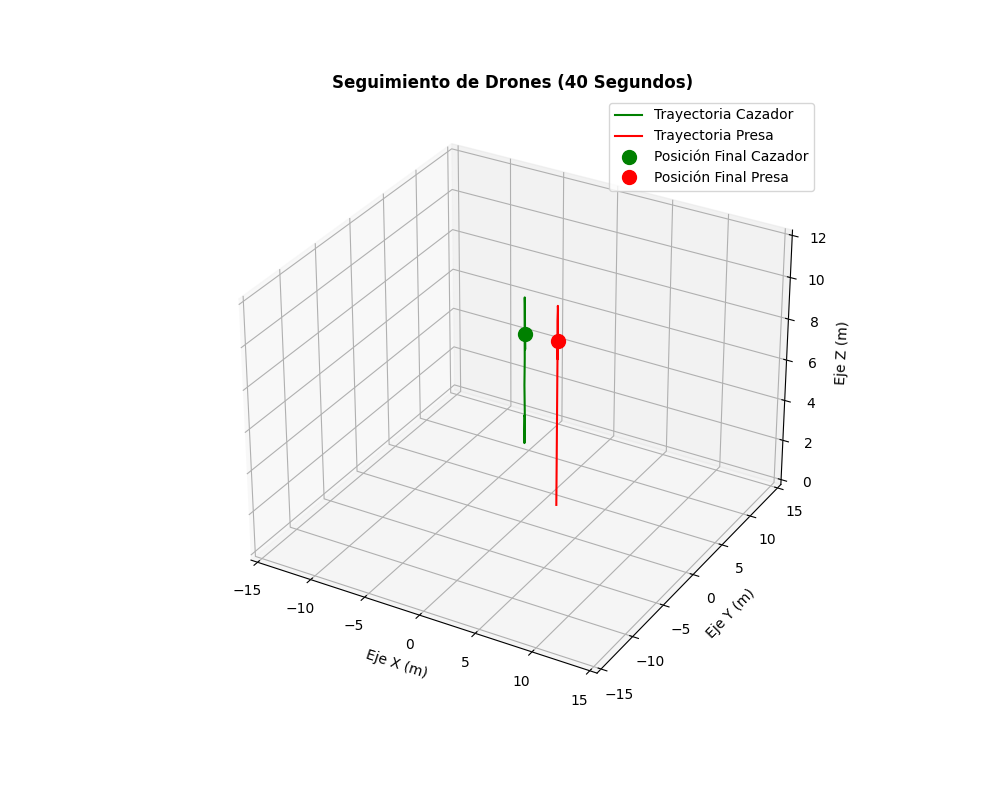
\includegraphics[width=1.0\textwidth]{imagenes/trayectoria3D-subir_bajar.png}
\caption{Trayectoria vertical utilizada para la prueba del PID de altura. (Imagen de Elaboración Propia)}
\label{fig:trayectoria-altura-subir-bajar}
\end{figure}

\vspace{0.3cm}

En la Figura \ref{fig:trayectoria-altura-subir-bajar} se observa que el movimiento del UAV objetivo se concentra en el eje vertical, mientras el UAV cazador permanece en una posición de referencia. Esta configuración permite analizar de forma directa la capacidad del controlador de altura para seguir movimientos ascendentes y descendentes del objetivo sin introducir cambios en el plano horizontal.

\vspace{0.3cm}

La respuesta del controlador se representa en la Figura \ref{fig:respuesta-pid-altura}. La señal verde corresponde al error vertical \texttt{Ey}, mientras que la línea roja discontinua marca la referencia de error nulo. A lo largo de la prueba, el error se mantiene en valores reducidos alrededor de cero, con pequeñas oscilaciones asociadas al movimiento sinusoidal del objetivo.

\begin{figure}[H]
\centering
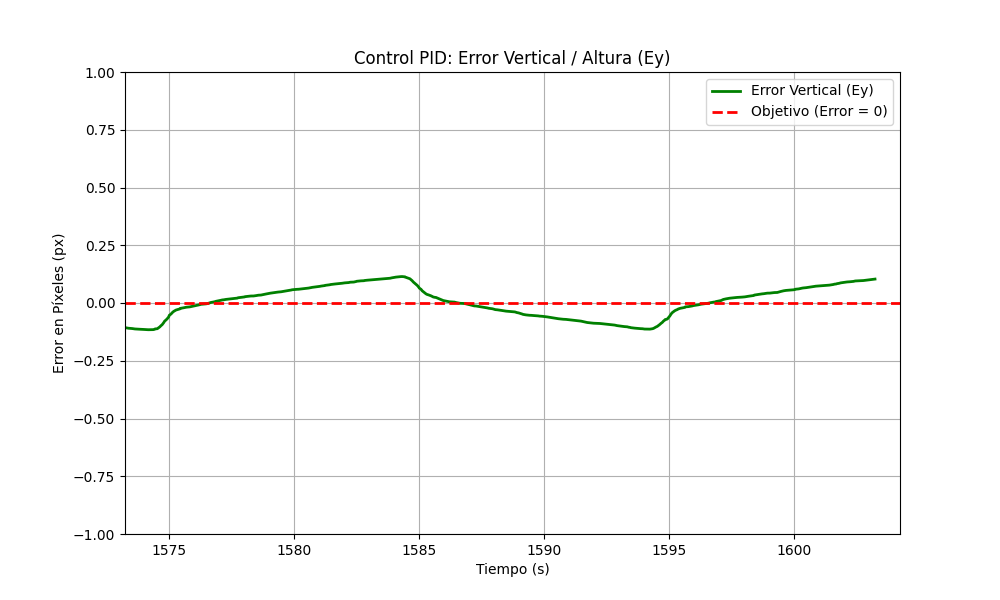
\includegraphics[width=0.95\textwidth]{imagenes/RespuestaPID_Altura.png}
\caption{Respuesta del PID de altura durante la trayectoria vertical. (Imagen de Elaboración Propia)}
\label{fig:respuesta-pid-altura}
\end{figure}

\vspace{0.3cm}

La evolución de la señal muestra que el controlador responde de forma suave ante las variaciones de altura. No aparecen oscilaciones crecientes ni sobreimpulsos elevados, y el error vertical permanece acotado durante toda la trayectoria. Aunque se aprecia una ligera desviación respecto a la referencia en algunos instantes, esta se corrige progresivamente y se mantiene dentro de un margen pequeño. Por tanto, la prueba confirma que el PID de altura es capaz de compensar los movimientos verticales del UAV objetivo y mantener una respuesta estable para el seguimiento visual.


\paragraph{Prueba del PID de distancia con trayectoria recta}\mbox{}\par

Esta prueba sirve para validar el PID de distancia, encargado de regular el avance longitudinal del UAV cazador respecto al UAV objetivo. La pregunta que se busca responder es si el dron cazador puede aproximarse y seguir a un objetivo en movimiento sin invadir la distancia de seguridad definida para el seguimiento.

\vspace{0.3cm}

El experimento consiste en hacer que el UAV objetivo siga una trayectoria recta a una velocidad constante de 3 m/s, avanzando un total aproximado de 25 metros. Durante esta maniobra, el controlador de distancia debe adaptar la velocidad frontal del UAV cazador para reducir la separación inicial y mantener una distancia longitudinal controlada.

\vspace{0.3cm}

Aunque el planteamiento general del TFG está orientado a tareas de interceptación, en las pruebas de validación se decidió no forzar una colisión ni un contacto directo entre ambos UAV. Esta decisión permite que los experimentos sean repetibles, comparables y más fáciles de trasladar posteriormente a pruebas reales. Por este motivo, el sistema se configuró para mantener una distancia de seguridad de 1 metro y medio respecto al UAV objetivo. De este modo, se evalúa la capacidad de aproximación y seguimiento sin comprometer la estabilidad de la simulación ni la seguridad de una posible plataforma física.

\vspace{0.3cm}

La trayectoria recta se generó desplazando progresivamente el UAV objetivo en una única dirección, manteniendo constante su altura y su orientación. Al imponer una velocidad de 3 m/s durante el recorrido, el controlador de distancia debe aumentar o reducir la velocidad frontal del UAV cazador para acercarse al objetivo y conservar la referencia deseada. Esta prueba resulta especialmente relevante porque combina una condición sencilla de analizar con una exigencia directa sobre el control longitudinal.

\begin{figure}[H]
\centering
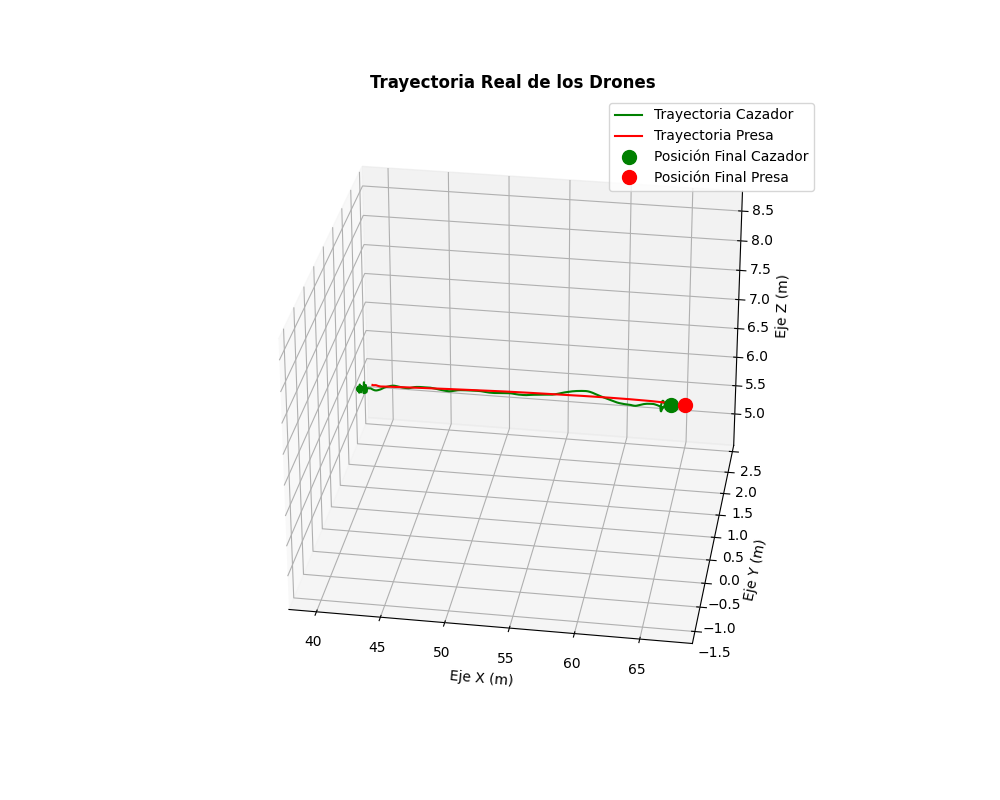
\includegraphics[width=1.0\textwidth]{imagenes/trayectoria3D-Recta.png}
\caption{Trayectoria recta utilizada para la prueba del PID de distancia. (Imagen de Elaboración Propia)}
\label{fig:trayectoria-recta-distancia}
\end{figure}

\vspace{0.3cm}

En la Figura \ref{fig:trayectoria-recta-distancia} se representa el desplazamiento rectilíneo del UAV objetivo y la respuesta del UAV cazador durante el seguimiento. La prueba permite observar si el controlador longitudinal es capaz de reducir la separación inicial y acompañar al objetivo durante el avance, manteniendo la distancia de seguridad establecida.

\vspace{0.3cm}

La respuesta del PID de distancia se muestra en la Figura \ref{fig:respuesta-pid-distancia}. En esta gráfica se analiza la evolución del error de distancia asociado a la diferencia entre la distancia estimada al objetivo y la distancia de referencia. Una respuesta adecuada debe tender hacia valores próximos a cero, lo que indica que el sistema ha alcanzado la separación deseada y que el UAV cazador acompaña al objetivo sin alejarse ni acercarse en exceso.

\begin{figure}[H]
\centering
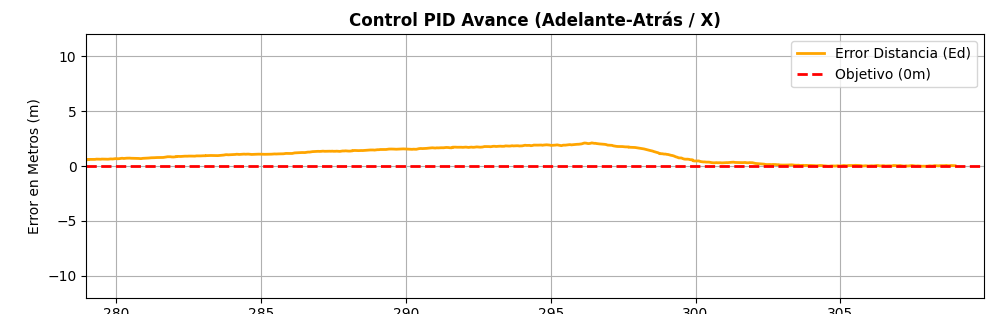
\includegraphics[width=0.95\textwidth]{imagenes/RespuestaPID_Distancia.png}
\caption{Respuesta del PID de distancia durante la trayectoria recta. (Imagen de Elaboración Propia)}
\label{fig:respuesta-pid-distancia}
\end{figure}

\vspace{0.3cm}

Los resultados muestran un comportamiento satisfactorio del controlador longitudinal. Tras el transitorio inicial, el error de distancia se reduce y permanece acotado, lo que indica que el UAV cazador es capaz de adaptarse al movimiento del objetivo a 3 m/s. Además, el seguimiento se realiza manteniendo la referencia de seguridad de 1 metro y medio, por lo que el sistema no solo se aproxima al objetivo, sino que también evita una interceptación directa. Esta respuesta confirma que el PID de distancia proporciona una base adecuada para escenarios de persecución controlada y para futuras pruebas reales donde la repetibilidad y la seguridad son requisitos fundamentales.

\subsubsection{Tiempos de establecimiento de los controladores PID}

Además de comprobar la estabilidad de cada controlador durante trayectorias continuas, se realizaron tres pruebas específicas para estimar su tiempo de establecimiento. Estas pruebas sirven para cuantificar la rapidez de respuesta de cada PID, no solo para observar si finalmente alcanza la referencia.

\vspace{0.3cm}

Con ellas se responde a la pregunta de cuánto tarda cada eje en reducir su error cuando parte de una desviación inicial conocida. Esta medida es importante porque, en un sistema de seguimiento visual, no basta con que el controlador sea estable: también debe reaccionar con suficiente rapidez para que el objetivo no salga del campo de visión.

\vspace{0.3cm}

El experimento consiste en colocar inicialmente el UAV cazador con un error controlado respecto al UAV objetivo y registrar el tiempo necesario para que la señal entre y permanezca dentro de una banda de tolerancia alrededor de la referencia. Para que los resultados fueran representativos del caso de uso del proyecto, las pruebas se plantearon con distancias cortas entre drones, ya que el sistema está orientado a seguimiento cercano del UAV objetivo y no a navegación a larga distancia.

\vspace{0.3cm}

En la prueba del PID de \textit{yaw}, el UAV cazador se situó inicialmente 1 metro desplazado hacia la izquierda respecto al objetivo, manteniendo una separación aproximada de 3 metros entre ambos drones. Esta configuración genera un error horizontal claro en la imagen sin introducir de forma dominante errores verticales o longitudinales. La respuesta obtenida se muestra en la Figura \ref{fig:pid-yaw-ts}.

\begin{figure}[H]
\centering
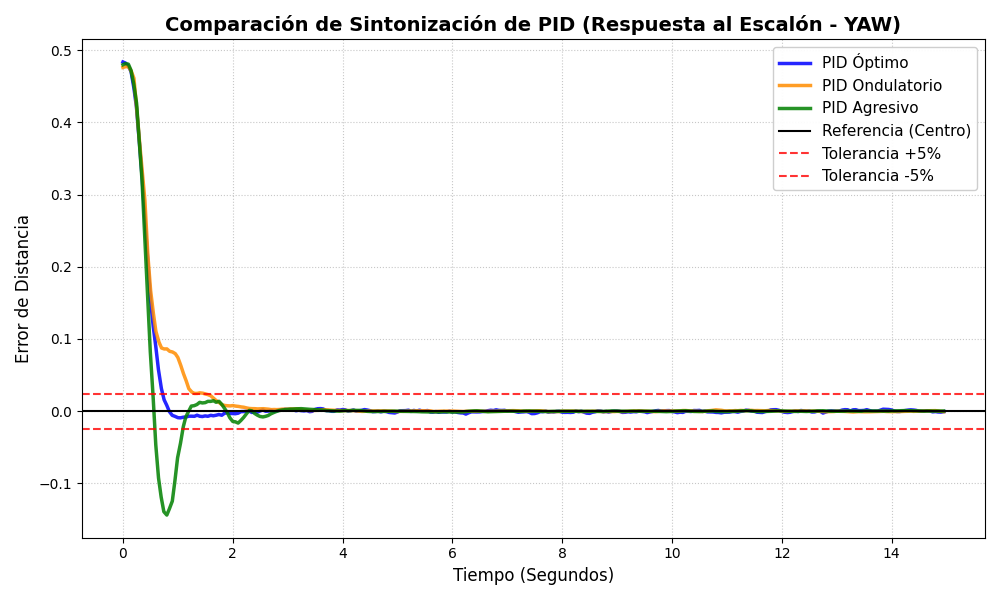
\includegraphics[width=0.95\textwidth]{imagenes/PID_YAW_Ts_V2.png}
\caption{Tiempo de establecimiento del PID de \textit{yaw}. (Imagen de Elaboración Propia)}
\label{fig:pid-yaw-ts}
\end{figure}

\vspace{0.3cm}

El tiempo de establecimiento obtenido para el PID de \textit{yaw} fue de aproximadamente $0.65\,\mathrm{s}$. Este valor es el menor de las tres pruebas porque la corrección de orientación se realiza mediante una velocidad angular, sin requerir un desplazamiento lineal completo del UAV cazador. Por ello, el sistema puede reducir rápidamente el error horizontal y centrar el objetivo en la imagen con una respuesta directa y poco oscilatoria.

\vspace{0.3cm}

En la prueba del PID de altura, el UAV cazador se colocó con un desfase vertical de 1 metro hacia arriba, manteniendo también una distancia aproximada de 3 metros respecto al UAV objetivo. Con esta configuración se fuerza un error vertical inicial que debe ser compensado por el controlador de altura, mientras que la separación cercana entre drones mantiene la prueba dentro del rango habitual de seguimiento visual. La respuesta se representa en la Figura \ref{fig:pid-altura-ts}.

\begin{figure}[H]
\centering
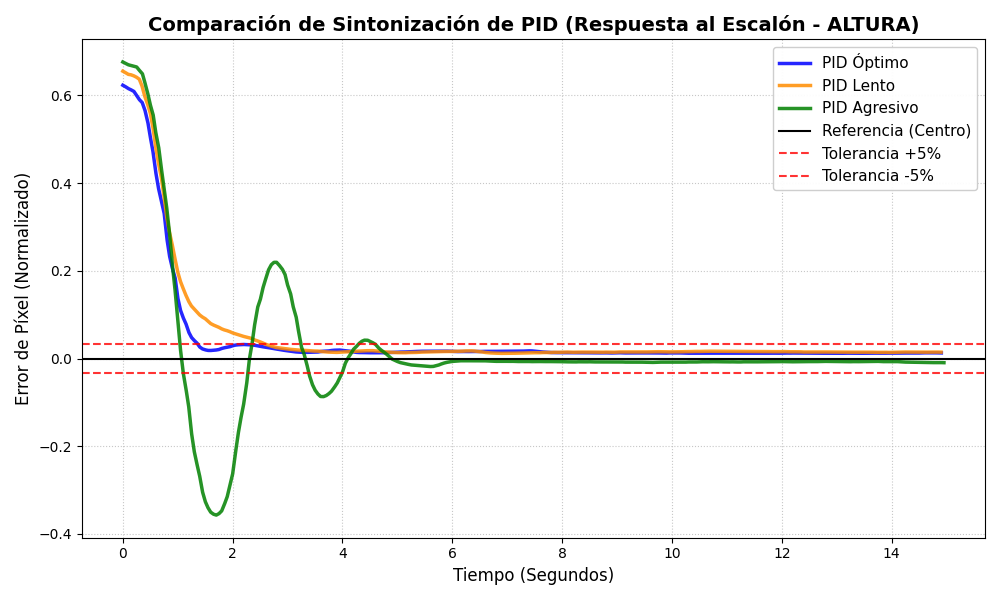
\includegraphics[width=0.95\textwidth]{imagenes/PID_Altura_Ts_V2.png}
\caption{Tiempo de establecimiento del PID de altura. (Imagen de Elaboración Propia)}
\label{fig:pid-altura-ts}
\end{figure}

\vspace{0.3cm}

El tiempo de establecimiento del PID de altura fue de aproximadamente $1.25\,\mathrm{s}$. Esta respuesta es más lenta que la del control de \textit{yaw} porque la corrección vertical depende del movimiento físico del UAV y de las limitaciones impuestas por el controlador de vuelo. Dichas limitaciones reducen la velocidad y la aceleración vertical máximas para evitar maniobras bruscas, por lo que el sistema tarda algo más en alcanzar la referencia, aunque mantiene una evolución estable y sin oscilaciones crecientes.

\vspace{0.3cm}

Por último, se evaluó el PID de distancia situando inicialmente los drones con una separación longitudinal de 3 metros. Esta prueba permite analizar la capacidad del controlador para regular el acercamiento al objetivo manteniendo una distancia de seguimiento segura. La elección de una distancia moderada responde a la necesidad de evitar choques entre drones y de hacer que la prueba sea repetible tanto en simulación como en una futura validación física. La respuesta se muestra en la Figura \ref{fig:pid-distancia-ts}.

\begin{figure}[H]
\centering
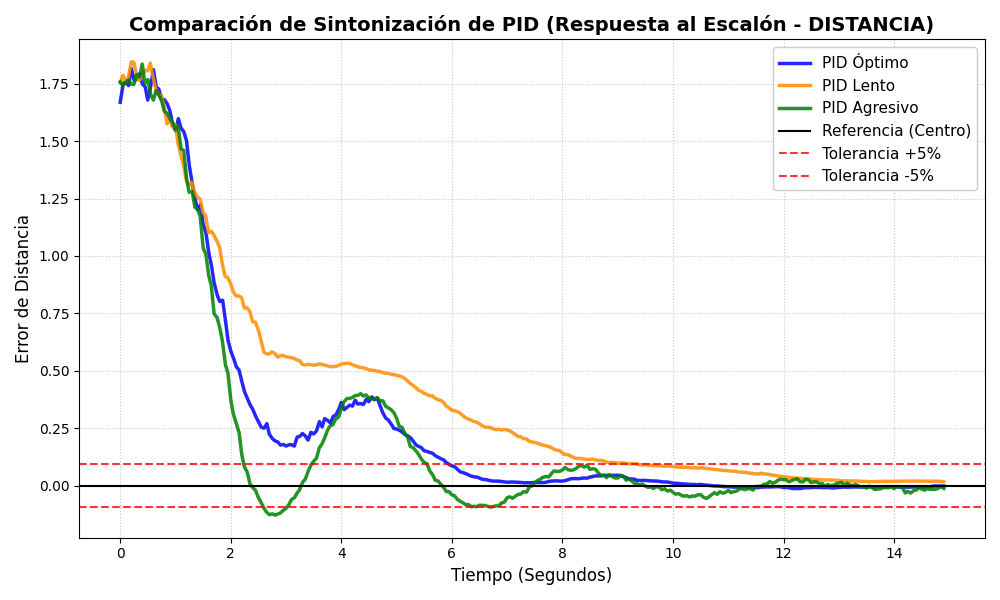
\includegraphics[width=0.95\textwidth]{imagenes/PID_DISTANCIA_Ts.png}
\caption{Tiempo de establecimiento del PID de distancia. (Imagen de Elaboración Propia)}
\label{fig:pid-distancia-ts}
\end{figure}

\vspace{0.3cm}

El tiempo de establecimiento del PID de distancia fue de aproximadamente $6\,\mathrm{s}$, notablemente superior al de los otros dos controladores. Este comportamiento se debe a que el avance longitudinal se ajustó de forma conservadora para no provocar una aproximación excesivamente agresiva al UAV objetivo. Además, debe tenerse en cuenta que este controlador PID está pensado para seguir a un UAV objetivo en movimiento, por lo que en una prueba estática aparece de forma más marcada la dinámica de aceleración y frenado frente a una referencia fija. Cuando el UAV cazador acelera para avanzar, tiende a inclinarse hacia delante; al frenar de forma brusca, realiza el movimiento contrario, generando un pequeño retroceso y variaciones en la estimación visual. Estas oscilaciones hacen que la señal tarde más en estabilizarse, pero también permiten mantener una maniobra más segura y reproducible, reduciendo el riesgo de colisión durante las pruebas.

\begin{table}[H]
\centering
\caption{Tiempos de establecimiento obtenidos para cada controlador PID.}
\label{tab:tiempos-establecimiento-pid}
\begin{tabular}{lcc}
\hline
\textbf{Controlador} & \textbf{Condición inicial} & \textbf{$T_s$} \\
\hline
PID de \textit{yaw} & 1 m lateral y 3 m de separación & $0.65\,\mathrm{s}$ \\
PID de altura & 1 m vertical y 3 m de separación & $1.25\,\mathrm{s}$ \\
PID de distancia & 3 m de separación longitudinal & $6\,\mathrm{s}$ \\
\hline
\end{tabular}
\end{table}

\vspace{0.3cm}

En conjunto, estos resultados muestran que los controladores lateral y vertical alcanzan la referencia en tiempos reducidos, mientras que el control de distancia presenta una respuesta más lenta debido a las restricciones de seguridad y a la propia dinámica longitudinal del UAV. Esta diferencia resulta aceptable para el sistema propuesto, ya que en un escenario de seguimiento cercano es preferible priorizar una aproximación suave y repetible antes que una reducción demasiado rápida de la distancia.

\subsubsection{Prueba conjunta de los tres PID activados en Simulación}

Una vez validados los controladores de forma individual, se realizó una prueba conjunta con los tres PID activados simultáneamente. Esta prueba sirve para comprobar si las acciones de \textit{yaw}, altura y distancia son compatibles cuando trabajan al mismo tiempo dentro del lazo de seguimiento visual.

\vspace{0.3cm}

Con este experimento se responde a la pregunta de si el sistema completo puede mantener errores acotados cuando el UAV objetivo genera desviaciones horizontales, verticales y longitudinales de manera simultánea. A diferencia de las pruebas anteriores, esta validación no aísla un único eje de control, sino que somete al sistema a una trayectoria tridimensional más exigente y cercana a una situación real de persecución.

\vspace{0.3cm}

El experimento consiste en activar los tres controladores y hacer que el UAV objetivo describa una trayectoria que combine movimiento circular en el plano horizontal con variaciones periódicas de altura. De esta forma, el UAV cazador debe corregir orientación, altura y avance de manera coordinada durante toda la maniobra.

\vspace{0.3cm}

La trayectoria del UAV objetivo se definió combinando un movimiento circular en el plano horizontal con una onda sinusoidal en altura. En el plano $XY$, el objetivo describe una circunferencia alrededor de un centro de referencia, utilizando una velocidad angular calculada a partir de la velocidad lineal y el radio de giro. Al mismo tiempo, la coordenada vertical se modifica mediante una onda de altura base $Z_0 = 7\,\mathrm{m}$, amplitud de $1\,\mathrm{m}$ y frecuencia de $0.1\,\mathrm{Hz}$. De este modo, la altura del objetivo varía de forma suave alrededor de los 7 metros, con un periodo aproximado de 10 segundos.

\vspace{0.3cm}

Esta configuración permite que el UAV objetivo avance alrededor del cazador mientras asciende y desciende periódicamente. La posición se actualizó a 20 Hz, manteniendo una orientación fija durante la trayectoria, de forma que las variaciones observadas por el sistema provinieran principalmente del movimiento espacial del objetivo. Con ello se buscó evaluar la coordinación entre el PID de \textit{yaw}, encargado del centrado horizontal, el PID de altura, responsable de corregir el error vertical, y el PID de distancia, encargado de mantener la separación longitudinal respecto al objetivo.

\begin{figure}[H]
\centering
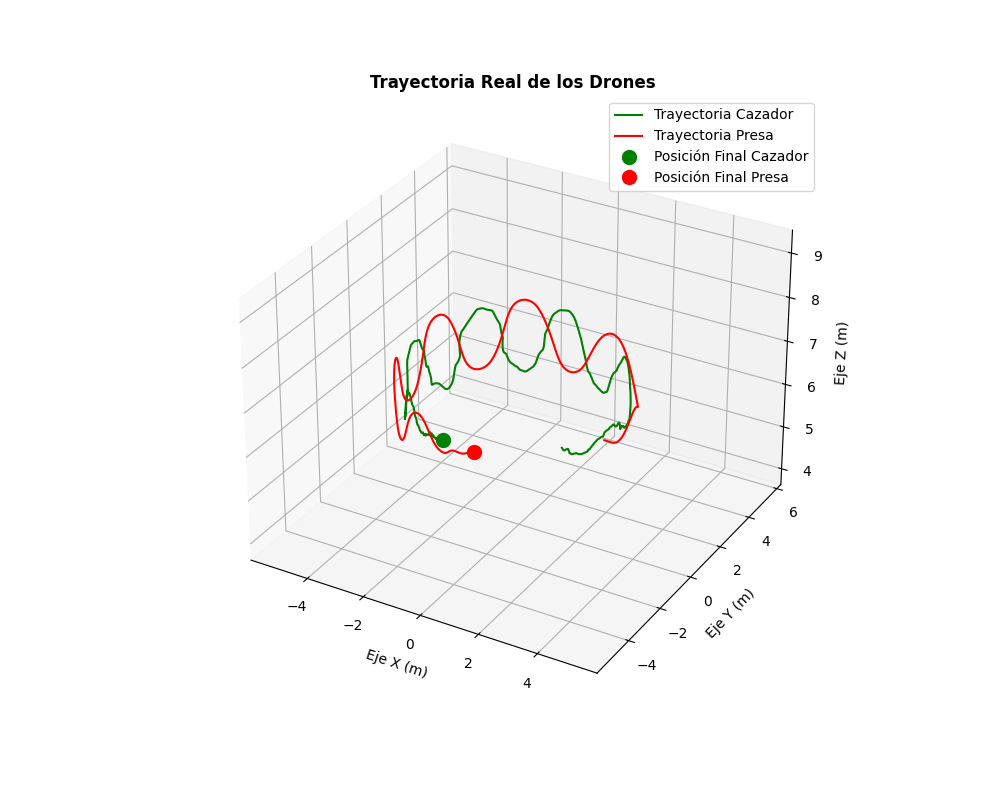
\includegraphics[width=1.0\textwidth]{imagenes/trayectoria3D-Total.png}
\caption{Trayectoria circular ondulada utilizada para la prueba conjunta de los tres PID. (Imagen de Elaboración Propia)}
\label{fig:trayectoria-total-pid}
\end{figure}

\vspace{0.3cm}

En la Figura \ref{fig:trayectoria-total-pid} se muestra la trayectoria tridimensional utilizada en la prueba. Se observa que el UAV objetivo no solo se desplaza en círculo, sino que también modifica su altura de forma continua. Esta combinación obliga al UAV cazador a corregir simultáneamente su orientación, su posición vertical y su avance, por lo que resulta adecuada para comprobar el funcionamiento conjunto del sistema de control visual.

\vspace{0.3cm}

La respuesta obtenida durante la ejecución se representa en la Figura \ref{fig:respuesta-pid-total}. En esta gráfica se analiza la evolución de las señales asociadas a los tres controladores cuando trabajan de manera simultánea. Una respuesta adecuada debe mantener los errores acotados, evitar oscilaciones crecientes y permitir que el UAV cazador conserve el seguimiento visual del objetivo a pesar de que la trayectoria introduce cambios continuos en los tres ejes.

\begin{figure}[H]
\centering
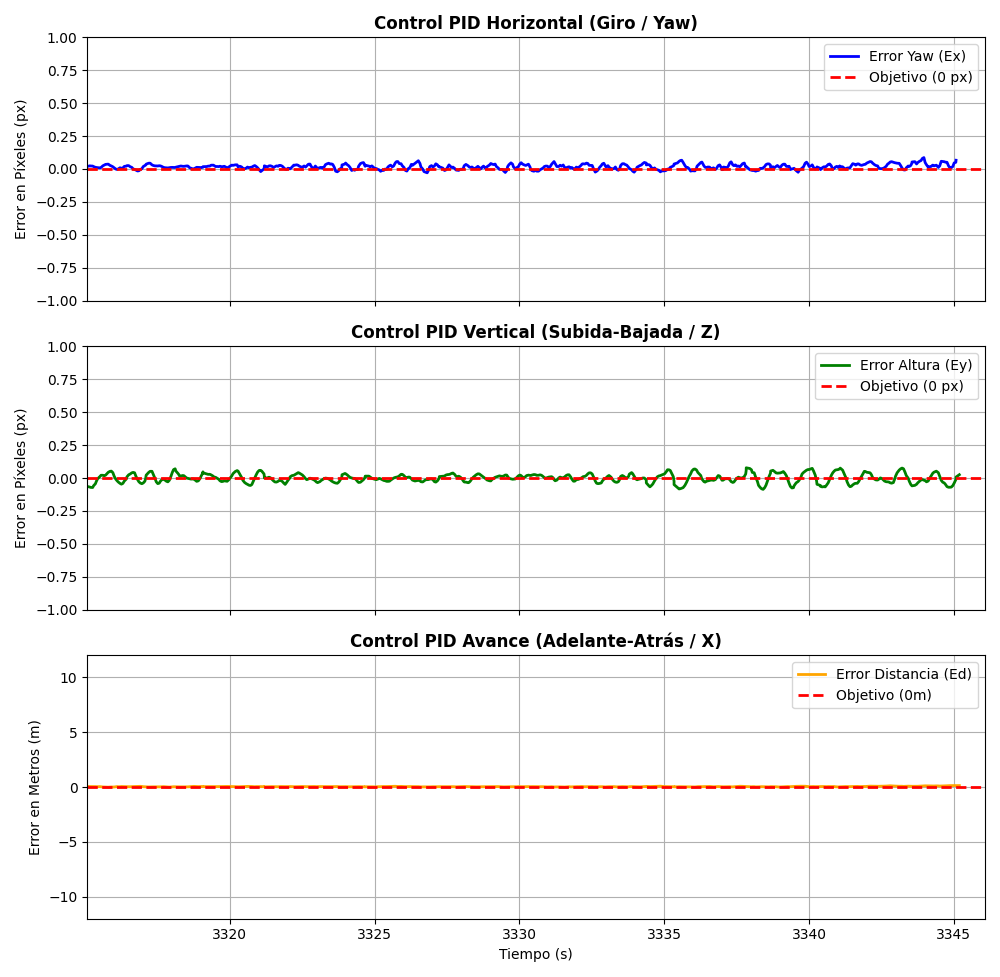
\includegraphics[width=0.95\textwidth]{imagenes/RespuestaPID_Total.png}
\caption{Respuesta conjunta de los tres PID durante la trayectoria circular ondulada. (Imagen de Elaboración Propia)}
\label{fig:respuesta-pid-total}
\end{figure}

\vspace{0.3cm}

Los resultados muestran que el sistema es capaz de mantener una respuesta estable cuando los tres controladores actúan a la vez. El PID de \textit{yaw} corrige el desplazamiento horizontal producido por el movimiento circular, el PID de altura compensa la variación sinusoidal de la coordenada vertical y el PID de distancia ajusta el avance del UAV cazador para conservar la separación de seguimiento. Aunque la trayectoria genera perturbaciones continuas y pequeñas oscilaciones en las señales de control, estas permanecen acotadas y no derivan en una pérdida del objetivo. Por tanto, esta prueba confirma que la integración de los tres PID permite abordar un escenario de seguimiento tridimensional más completo que las validaciones individuales.



\clearpage

\subsection{Seguimiento del Objetivo en Simulación}

Estas pruebas sirven para validar el comportamiento del sistema cuando el UAV presa realiza trayectorias completas y el UAV cazador debe mantener el seguimiento durante un vuelo continuo. A diferencia de las validaciones individuales de los PID, aquí no se evalúa un controlador aislado, sino la integración de percepción, estimación y control.

\vspace{0.3cm}

Con este bloque se responde a la pregunta de si el sistema completo puede conservar una referencia visual útil cuando el objetivo cambia de posición de forma dinámica. Por ello se analizan las métricas de visión, como la detección directa de YOLO, el apoyo del filtro de Kalman y la tasa de pérdida del objetivo, junto con métricas de control como el EPE de centrado y el RMSE de distancia.

\vspace{0.3cm}

Los experimentos consisten en ejecutar tres escenarios progresivos en simulación: una trayectoria en zigzag, una trayectoria circular ondulada y una ruta final definida por \textit{waypoints}. En todos los casos se registran los frames analizados, el porcentaje de detección directa, el uso de Kalman, el TLR, el error de centrado y el error de distancia para, posteriormente, exponer los resultados y discutir las limitaciones observadas.

\subsubsection{Prueba de seguimiento con trayectoria en zigzag}

Esta prueba sirve para evaluar el seguimiento visual ante cambios laterales sucesivos. La trayectoria en zigzag obliga al UAV cazador a corregir alternancias en el error horizontal mientras intenta mantener la distancia de referencia y el centrado vertical del objetivo.

\vspace{0.3cm}

Con este experimento se responde a la pregunta de si el sistema puede mantener la referencia visual sin depender de una trayectoria suave o rectilínea. Es una prueba relevante porque los cambios de dirección pueden provocar desplazamientos rápidos de la caja detectada, variaciones en la estimación de distancia y posibles pérdidas temporales de detección.

\vspace{0.3cm}

El experimento consiste en hacer que el UAV presa realice un desplazamiento en zigzag mientras el UAV cazador intenta mantenerlo dentro del campo de visión. Durante el vuelo permanecen activos los tres controladores principales: el PID de \textit{yaw}, encargado de corregir el error horizontal de la imagen; el PID de altura, responsable de reducir el error vertical; y el PID de distancia, utilizado para regular la separación longitudinal respecto al objetivo.

\vspace{0.3cm}

La trayectoria utilizada se muestra en la Figura \ref{fig:trayectoria-zigzag-seguimiento}. El movimiento alterna desplazamientos laterales a medida que el objetivo avanza, generando cambios de signo en el error horizontal. Esta característica permite comprobar si el controlador de \textit{yaw} responde con suficiente rapidez y si el detector mantiene una localización estable del UAV presa durante los cambios de dirección.

\begin{figure}[H]
\centering
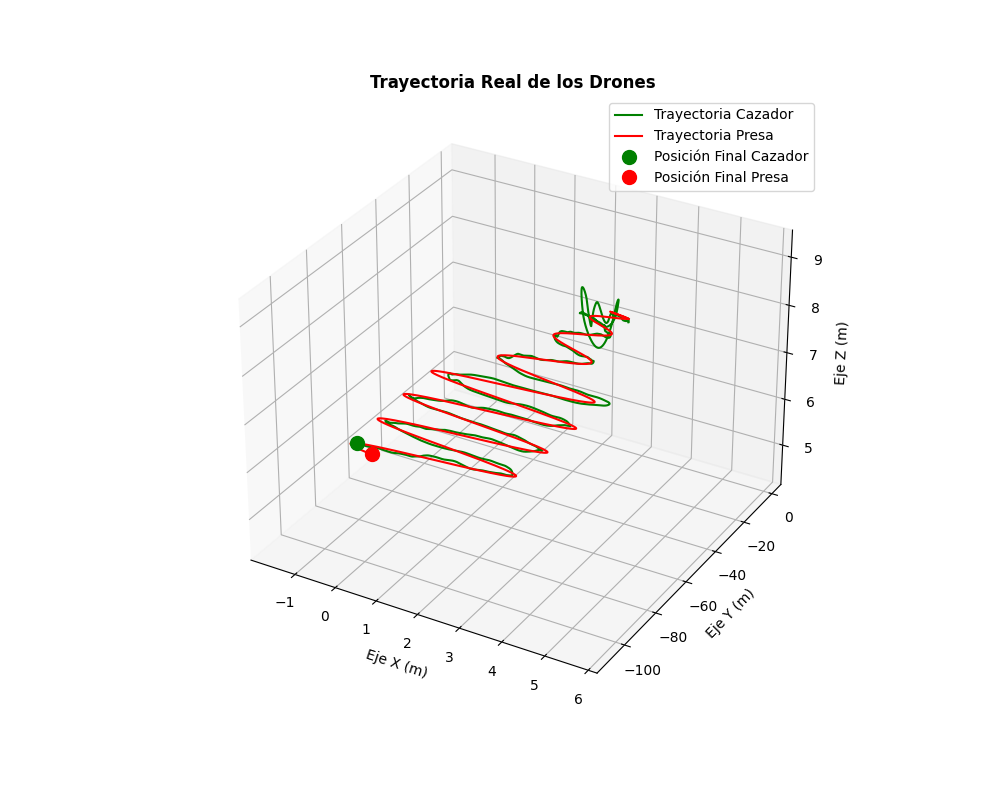
\includegraphics[width=1.0\textwidth]{imagenes/Trayectoria_ZigZag.png}
\caption{Trayectoria en zigzag utilizada para la prueba de seguimiento del objetivo. (Imagen de Elaboración Propia)}
\label{fig:trayectoria-zigzag-seguimiento}
\end{figure}

\vspace{0.3cm}

La Figura \ref{fig:gazebo-drones-zigzag} muestra una vista del escenario de Gazebo durante esta prueba, con ambos UAV dentro del entorno de simulación utilizado para evaluar el seguimiento.

\begin{figure}[H]
\centering
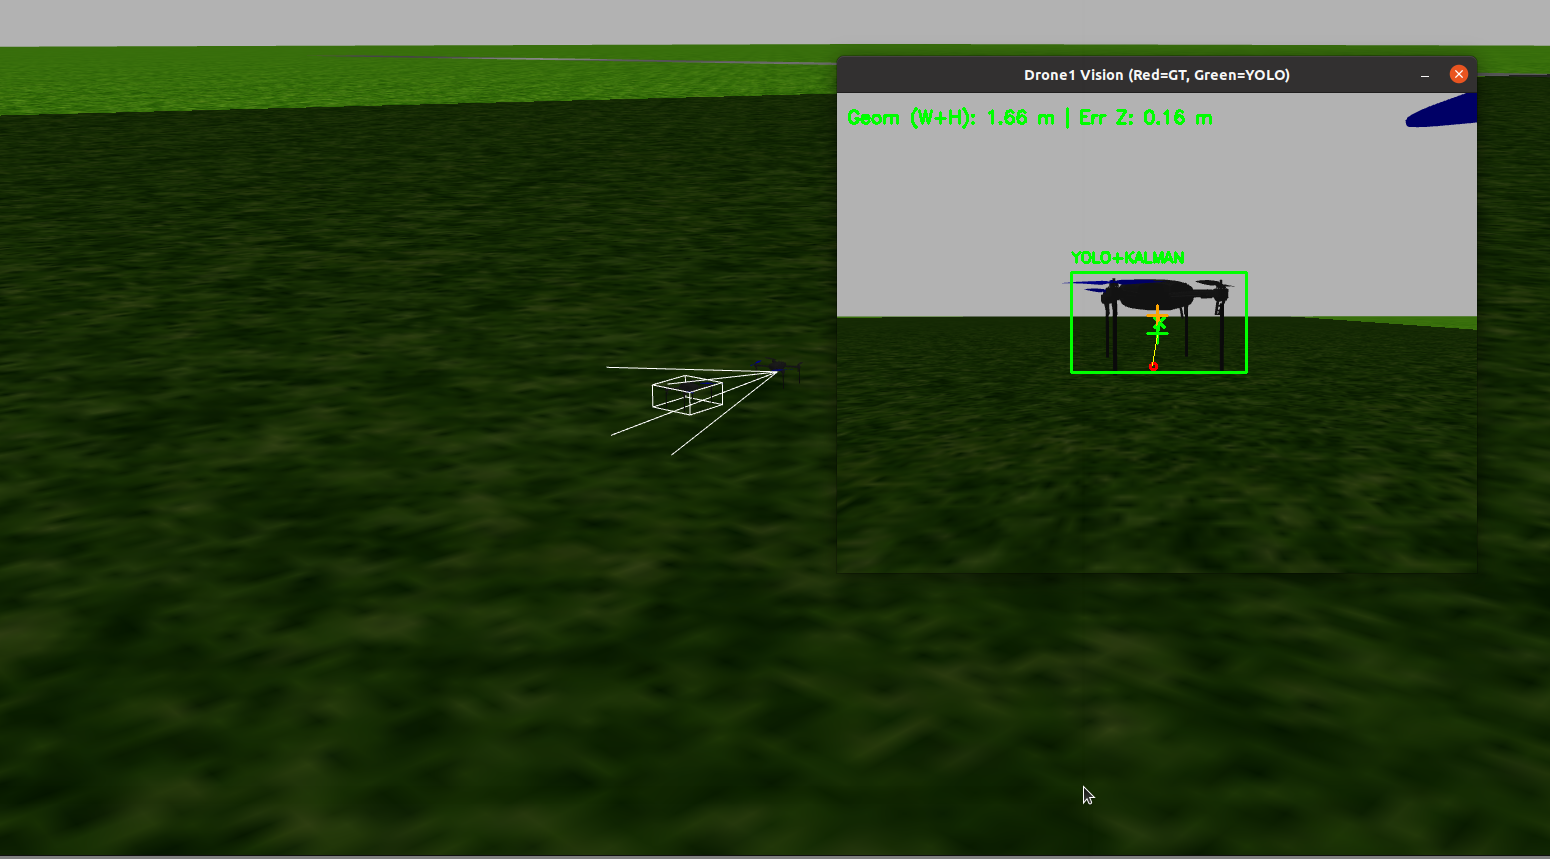
\includegraphics[width=0.95\textwidth]{imagenes/gazeboDrones2.png}
\caption{Vista del escenario de Gazebo y la camara durante la prueba de seguimiento en zigzag. (Imagen de Elaboración Propia)}
\label{fig:gazebo-drones-zigzag}
\end{figure}

\vspace{0.3cm}

Durante la ejecución se registraron las señales del evaluador de métricas del vuelo. El informe final obtenido se resume en la Tabla \ref{tab:metricas-seguimiento-zigzag}. En ella se recogen las métricas de visión, el EPE 2D de centrado en imagen y el RMSE de distancia, manteniendo separadas las pérdidas de percepción respecto al error de control.

\begin{table}[H]
\centering
\caption{Métricas EPE/RMSE/TLR obtenidas durante la prueba de seguimiento con trayectoria en zigzag.}
\label{tab:metricas-seguimiento-zigzag}
\begin{tabular}{lc}
\hline
\textbf{Métrica} & \textbf{Valor} \\
\hline
Frames analizados & 3266 \\
Visión activa con YOLO & $100.00\%$ \\
\textit{Tracking} ciego con Kalman & $0.00\%$ \\
\textit{Target Loss Rate} (TLR) & $0.00\%$ \\
EPE durante YOLO & 0.0550 normalizado \\
EPE durante Kalman & No aplicable \\
EPE medio total & 0.0550 normalizado \\
RMSE de distancia ($E_z$) & $1.255\,\mathrm{m}$ \\
\hline
\end{tabular}
\end{table}

\vspace{0.3cm}

Los resultados de visión muestran que el sistema mantuvo detección directa durante toda la maniobra. De los 3266 frames analizados, YOLO proporcionó una referencia válida en el $100.00\%$ de los casos, no fue necesario recurrir a la predicción de la caja mediante Kalman y el TLR se mantuvo en $0.00\%$. Por tanto, no se produjo ninguna pérdida completa del objetivo durante el vuelo.

\vspace{0.3cm}

El EPE medio total fue de 0.0550 en magnitud normalizada, calculado íntegramente durante frames con detección YOLO. Este valor resume el error bidimensional de centrado en la imagen, combinando las componentes horizontal y vertical. Al no haberse usado Kalman, el EPE asociado a este modo se considera no aplicable, lo que refuerza que el seguimiento visual dependió de detecciones directas durante toda la prueba.

\vspace{0.3cm}

El RMSE de distancia fue de $1.255\,\mathrm{m}$. Este valor indica que la separación longitudinal fue la componente más difícil de mantener durante la trayectoria en zigzag. Los cambios laterales sucesivos modifican la posición relativa entre ambos UAV y pueden introducir variaciones en la estimación de profundidad basada en la caja delimitadora, por lo que el error de distancia resulta mayor que los errores normalizados de centrado visual.

\vspace{0.3cm}

En conjunto, la prueba de zigzag confirma que el sistema es capaz de mantener la referencia visual del UAV presa en una trayectoria con cambios laterales sucesivos. Aunque el control de distancia presenta un error mayor que los ejes de centrado visual, la detección se mantiene estable durante toda la secuencia y no se produce pérdida del objetivo.

\subsubsection{Prueba de seguimiento con trayectoria circular ondulada}

Esta prueba sirve para evaluar el seguimiento cuando el objetivo genera errores simultáneos en \textit{yaw}, altura y distancia. La trayectoria circular ondulada combina desplazamiento circular en el plano horizontal con variaciones sinusoidales de altura, por lo que representa una maniobra tridimensional más completa que el zigzag.

\vspace{0.3cm}

Con este experimento se responde a la pregunta de si la validación conjunta de los tres PID se mantiene también desde el punto de vista de la continuidad visual. Es decir, no solo se comprueba que los controladores puedan actuar de forma simultánea, sino también que la percepción proporcione una referencia suficientemente estable durante toda la maniobra.

\vspace{0.3cm}

El experimento consiste en reutilizar la trayectoria circular ondulada mostrada previamente en la Figura \ref{fig:trayectoria-total-pid} y registrar métricas específicas de seguimiento. Para ello se recogieron las métricas EPE/RMSE/TLR del vuelo, incluyendo el error de centrado bidimensional, el error de distancia y los porcentajes de detección directa, seguimiento mediante Kalman y pérdida del objetivo.

\vspace{0.3cm}

La Figura \ref{fig:gazebo-drones-circular} muestra la escena de Gazebo correspondiente a esta segunda prueba de seguimiento, donde el UAV cazador mantiene la referencia visual del UAV objetivo durante la maniobra circular ondulada.

\begin{figure}[H]
\centering
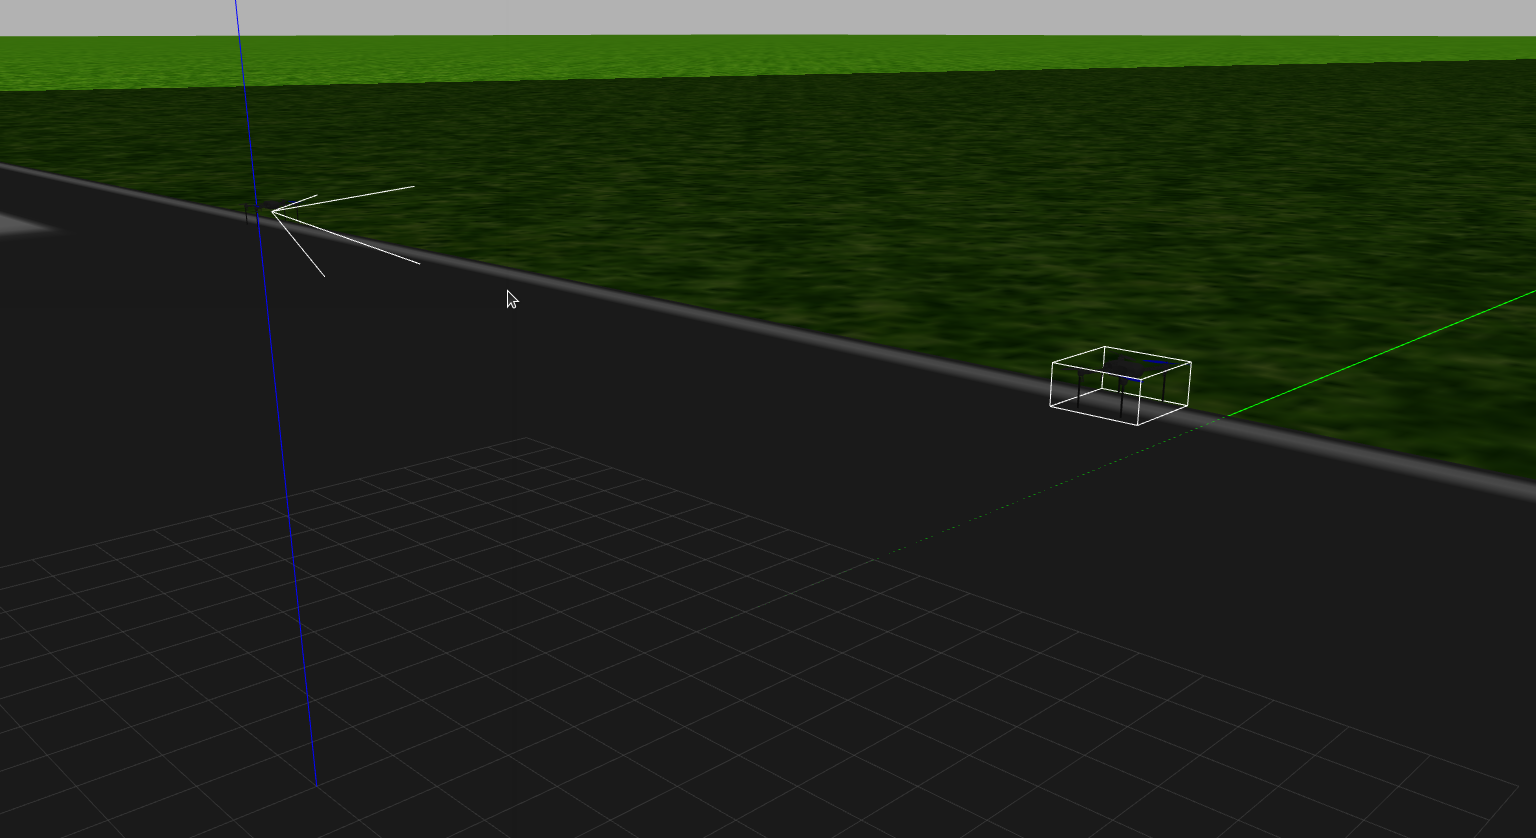
\includegraphics[width=0.95\textwidth]{imagenes/GazeboDrones.png}
\caption{Vista del escenario incial de Gazebo  en  la prueba de seguimiento con trayectoria circular ondulada. (Imagen de Elaboración Propia)}
\label{fig:gazebo-drones-circular}
\end{figure}

\vspace{0.3cm}

Los resultados obtenidos se resumen en la Tabla \ref{tab:metricas-seguimiento-total}. Al igual que en la prueba anterior, los errores de imagen y el error de distancia se presentan por separado, ya que corresponden a magnitudes con unidades distintas.

\begin{table}[H]
\centering
\caption{Métricas EPE/RMSE/TLR obtenidas durante la prueba de seguimiento con trayectoria circular ondulada.}
\label{tab:metricas-seguimiento-total}
\begin{tabular}{lc}
\hline
\textbf{Métrica} & \textbf{Valor} \\
\hline
Frames analizados & 6499 \\
Visión activa con YOLO & $99.74\%$ \\
\textit{Tracking} ciego con Kalman & $0.26\%$ \\
\textit{Target Loss Rate} (TLR) & $0.00\%$ \\
EPE durante YOLO & 0.0510 normalizado \\
EPE durante Kalman & 0.1590 normalizado \\
EPE medio total & 0.0513 normalizado \\
RMSE de distancia ($E_z$) & $0.2200\,\mathrm{m}$ \\
\hline
\end{tabular}
\end{table}

\vspace{0.3cm}

Los resultados de seguimiento muestran un centrado preciso durante la trayectoria circular ondulada. El EPE medio total fue de 0.0513 en magnitud normalizada, con un valor de 0.0510 durante los frames con detección directa de YOLO. En los instantes en los que fue necesario recurrir al seguimiento ciego mediante Kalman, el EPE aumentó hasta 0.1590, lo que indica que la predicción mantiene una referencia útil, aunque con menor precisión que la detección directa.

\vspace{0.3cm}

Desde el punto de vista de la visión, el detector YOLO mantuvo detección directa en el $99.74\%$ de los 6499 frames analizados. En el $0.26\%$ restante fue necesario recurrir al seguimiento predictivo mediante el filtro de Kalman, pero el TLR se mantuvo en $0.00\%$. Esto indica que, aunque aparecen interrupciones muy puntuales de la detección directa, el sistema no pierde completamente la referencia del UAV objetivo durante la maniobra.

\vspace{0.3cm}

El RMSE de distancia fue de $0.2200\,\mathrm{m}$, muy inferior al obtenido en la prueba de zigzag. Esto indica que, en esta trayectoria, el sistema mantuvo con mayor precisión la separación longitudinal respecto al UAV objetivo. En conjunto, la prueba confirma que la trayectoria circular ondulada no solo es útil para validar la actuación simultánea de los tres PID, sino también para medir la robustez del seguimiento visual en una situación tridimensional. La combinación de un TLR nulo, una detección directa superior al $99\%$ y errores EPE/RMSE reducidos demuestra que el sistema mantiene una referencia visual estable incluso cuando el objetivo introduce cambios simultáneos en el plano horizontal, la altura y la distancia.

\subsubsection{Prueba de seguimiento con ruta final por \textit{waypoints}}

Esta prueba sirve como validación final del seguimiento en simulación. A diferencia de las trayectorias anteriores, la ruta por \textit{waypoints} no sigue una forma periódica simple, sino que combina desplazamientos largos en el plano horizontal con cambios de altura entre puntos consecutivos.

\vspace{0.3cm}

Con este experimento se responde a la pregunta de si el sistema conserva la referencia visual en una maniobra menos regular y más representativa de un seguimiento general. En esta versión, la ruta aumenta el recorrido longitudinal y presenta un tramo final más prolongado, por lo que el UAV presa realiza una maniobra más exigente en la que el UAV cazador debe mantener el objetivo visible mientras cambian simultáneamente la posición lateral, longitudinal y vertical.

\vspace{0.3cm}

El experimento consiste en definir una secuencia de \textit{waypoints} y hacer que el UAV presa los recorra dentro del entorno de simulación. Los puntos utilizados para generar la trayectoria se recogen en la Tabla \ref{tab:waypoints-ruta-final}; cada \textit{waypoint} está definido mediante sus coordenadas $(x,y,z)$ en metros.

\begin{table}[H]
\centering
\caption{\textit{Waypoints} utilizados en la ruta final de seguimiento.}
\label{tab:waypoints-ruta-final}
\begin{tabular}{lccc}
\hline
\textbf{Punto} & \textbf{$x$ (m)} & \textbf{$y$ (m)} & \textbf{$z$ (m)} \\
\hline
WP0 & 5.0  & $-30.0$ & 8.0 \\
WP1 & 15.0 & $-20.0$ & 5.0 \\
WP2 & 35.0 & $-25.0$ & 12.0 \\
WP3 & 40.0 & 20.0   & 9.0 \\
WP4 & 25.0 & 25.0   & 15.0 \\
WP5 & 35.0 & 80.0   & 15.0 \\
\hline
\end{tabular}
\end{table}

\vspace{0.3cm}

La trayectoria resultante se muestra en la Figura \ref{fig:trayectoria-final-seguimiento}. La ruta obliga al sistema a adaptarse a varios tramos con cambios de dirección y altura, incluyendo un desplazamiento final largo hasta $y=80\,\mathrm{m}$. Por ello, resulta adecuada para cerrar el bloque de pruebas de seguimiento con un escenario menos regular que el zigzag o la trayectoria circular ondulada.

\begin{figure}[H]
\centering
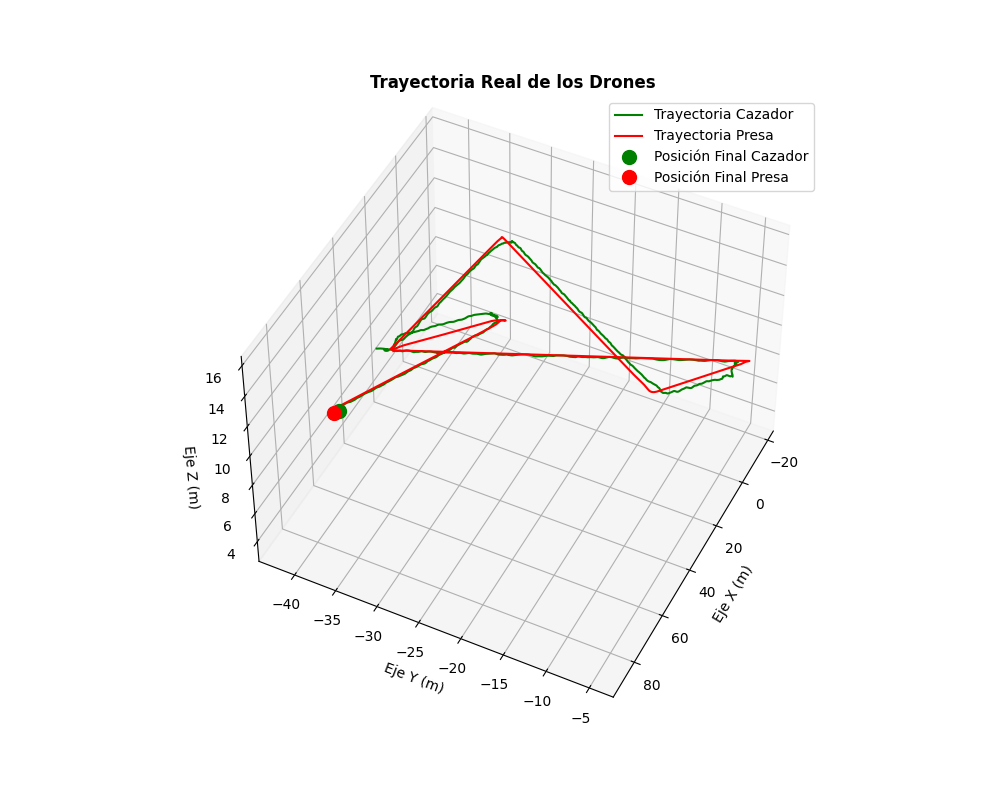
\includegraphics[width=1.0\textwidth]{imagenes/taryectoria_final.png}
\caption{Trayectoria final por \textit{waypoints} utilizada para la prueba de seguimiento. (Imagen de Elaboración Propia)}
\label{fig:trayectoria-final-seguimiento}
\end{figure}

\vspace{0.3cm}

Durante la ejecución se registraron las métricas EPE/RMSE/TLR del vuelo. Los resultados obtenidos se resumen en la Tabla \ref{tab:metricas-seguimiento-final}.

\begin{table}[H]
\centering
\caption{Métricas EPE/RMSE/TLR obtenidas durante la prueba de seguimiento con ruta final por \textit{waypoints}.}
\label{tab:metricas-seguimiento-final}
\begin{tabular}{lc}
\hline
\textbf{Métrica} & \textbf{Valor} \\
\hline
Frames analizados & 17911 \\
Visión activa con YOLO & $99.98\%$ \\
\textit{Tracking} ciego con Kalman & $0.03\%$ \\
\textit{Target Loss Rate} (TLR) & $0.00\%$ \\
EPE durante YOLO & 0.0221 normalizado \\
EPE durante Kalman & 0.0584 normalizado \\
EPE medio total & 0.0221 normalizado \\
RMSE de distancia ($E_z$) & $0.6821\,\mathrm{m}$ \\
\hline
\end{tabular}
\end{table}

\vspace{0.3cm}

Los resultados de visión muestran que el sistema mantuvo una detección directa prácticamente continua durante la ruta final. De los 17911 frames analizados, YOLO proporcionó una referencia válida en el $99.98\%$ de los casos, mientras que el filtro de Kalman solo fue necesario en un porcentaje residual, del $0.03\%$. Además, el TLR fue de $0.00\%$, por lo que no se produjo ninguna pérdida completa del objetivo durante la trayectoria.

\vspace{0.3cm}

El EPE medio total fue de 0.0221 en magnitud normalizada, coincidiendo tras el redondeo con el valor obtenido durante detección directa de YOLO debido al uso casi exclusivo de detecciones observadas. Durante los instantes puntuales en los que se recurrió a Kalman, el EPE fue de 0.0584, lo que indica que la predicción mantuvo una referencia suficientemente precisa incluso cuando no existía una caja observada por el detector. Este resultado supone una mejora clara respecto a las pruebas anteriores en términos de centrado visual.

\vspace{0.3cm}

El RMSE de distancia fue de $0.6821\,\mathrm{m}$. Este valor es mayor que el obtenido en la trayectoria circular ondulada, pero menor que el registrado en la prueba de zigzag. La diferencia se debe a que la ruta final introduce desplazamientos más largos entre \textit{waypoints} y cambios de altura que dificultan mantener constante la separación longitudinal. Aun así, el error permanece acotado y no afecta a la continuidad del seguimiento visual.

\vspace{0.3cm}

En conjunto, la ruta final confirma que el sistema puede mantener el seguimiento del UAV presa en una trayectoria tridimensional compuesta por varios tramos, cambios de altura y un recorrido longitudinal amplio. La combinación de una detección YOLO prácticamente continua, un uso muy reducido de Kalman, un TLR nulo y un EPE medio total bajo indica que el sistema de percepción y control conserva una referencia visual robusta incluso en una maniobra menos regular y más cercana a un escenario de seguimiento general.

\subsection{Prueba de Estimación de Distancia con Cámara Real}

Esta prueba sirve como primera validación real del sistema de estimación de distancia utilizando la cámara física y el UAV objetivo real. A diferencia de las pruebas en simulación, aquí la estimación depende de la calibración real de la cámara, de las dimensiones medidas del dron objetivo y de las variaciones propias de una detección visual en un entorno no ideal.

\vspace{0.3cm}

Con este experimento se responde a la pregunta de si la distancia calculada a partir de la caja delimitadora mantiene una relación coherente con la separación real entre la cámara y el dron objetivo. También permite estudiar el límite práctico del sistema de percepción, identificando a partir de qué rango la estimación empieza a degradarse por el menor tamaño aparente del UAV en la imagen.

\vspace{0.3cm}

El experimento consiste en realizar capturas a distintas distancias conocidas, comenzando por separaciones cercanas, donde el UAV ocupa una parte significativa de la imagen, y aumentando progresivamente la separación hasta distancias mayores. La prueba se repitió cinco veces para obtener resultados más consistentes y evaluar la dispersión entre mediciones, ya que una variación de pocos píxeles en la caja delimitadora puede traducirse en un cambio significativo en la distancia, especialmente cuando el UAV objetivo se encuentra más alejado.

\vspace{0.3cm}

El montaje experimental empleado para esta prueba se muestra en la Figura \ref{fig:dron-prueba-distancia}. En él se situó el dron objetivo frente a la cámara del dron cazador y se utilizó un metro como referencia física para ir colocando el UAV a distintas separaciones conocidas. De esta forma fue posible comparar la distancia real medida manualmente con la distancia estimada por el sistema.

\begin{figure}[H]
\centering
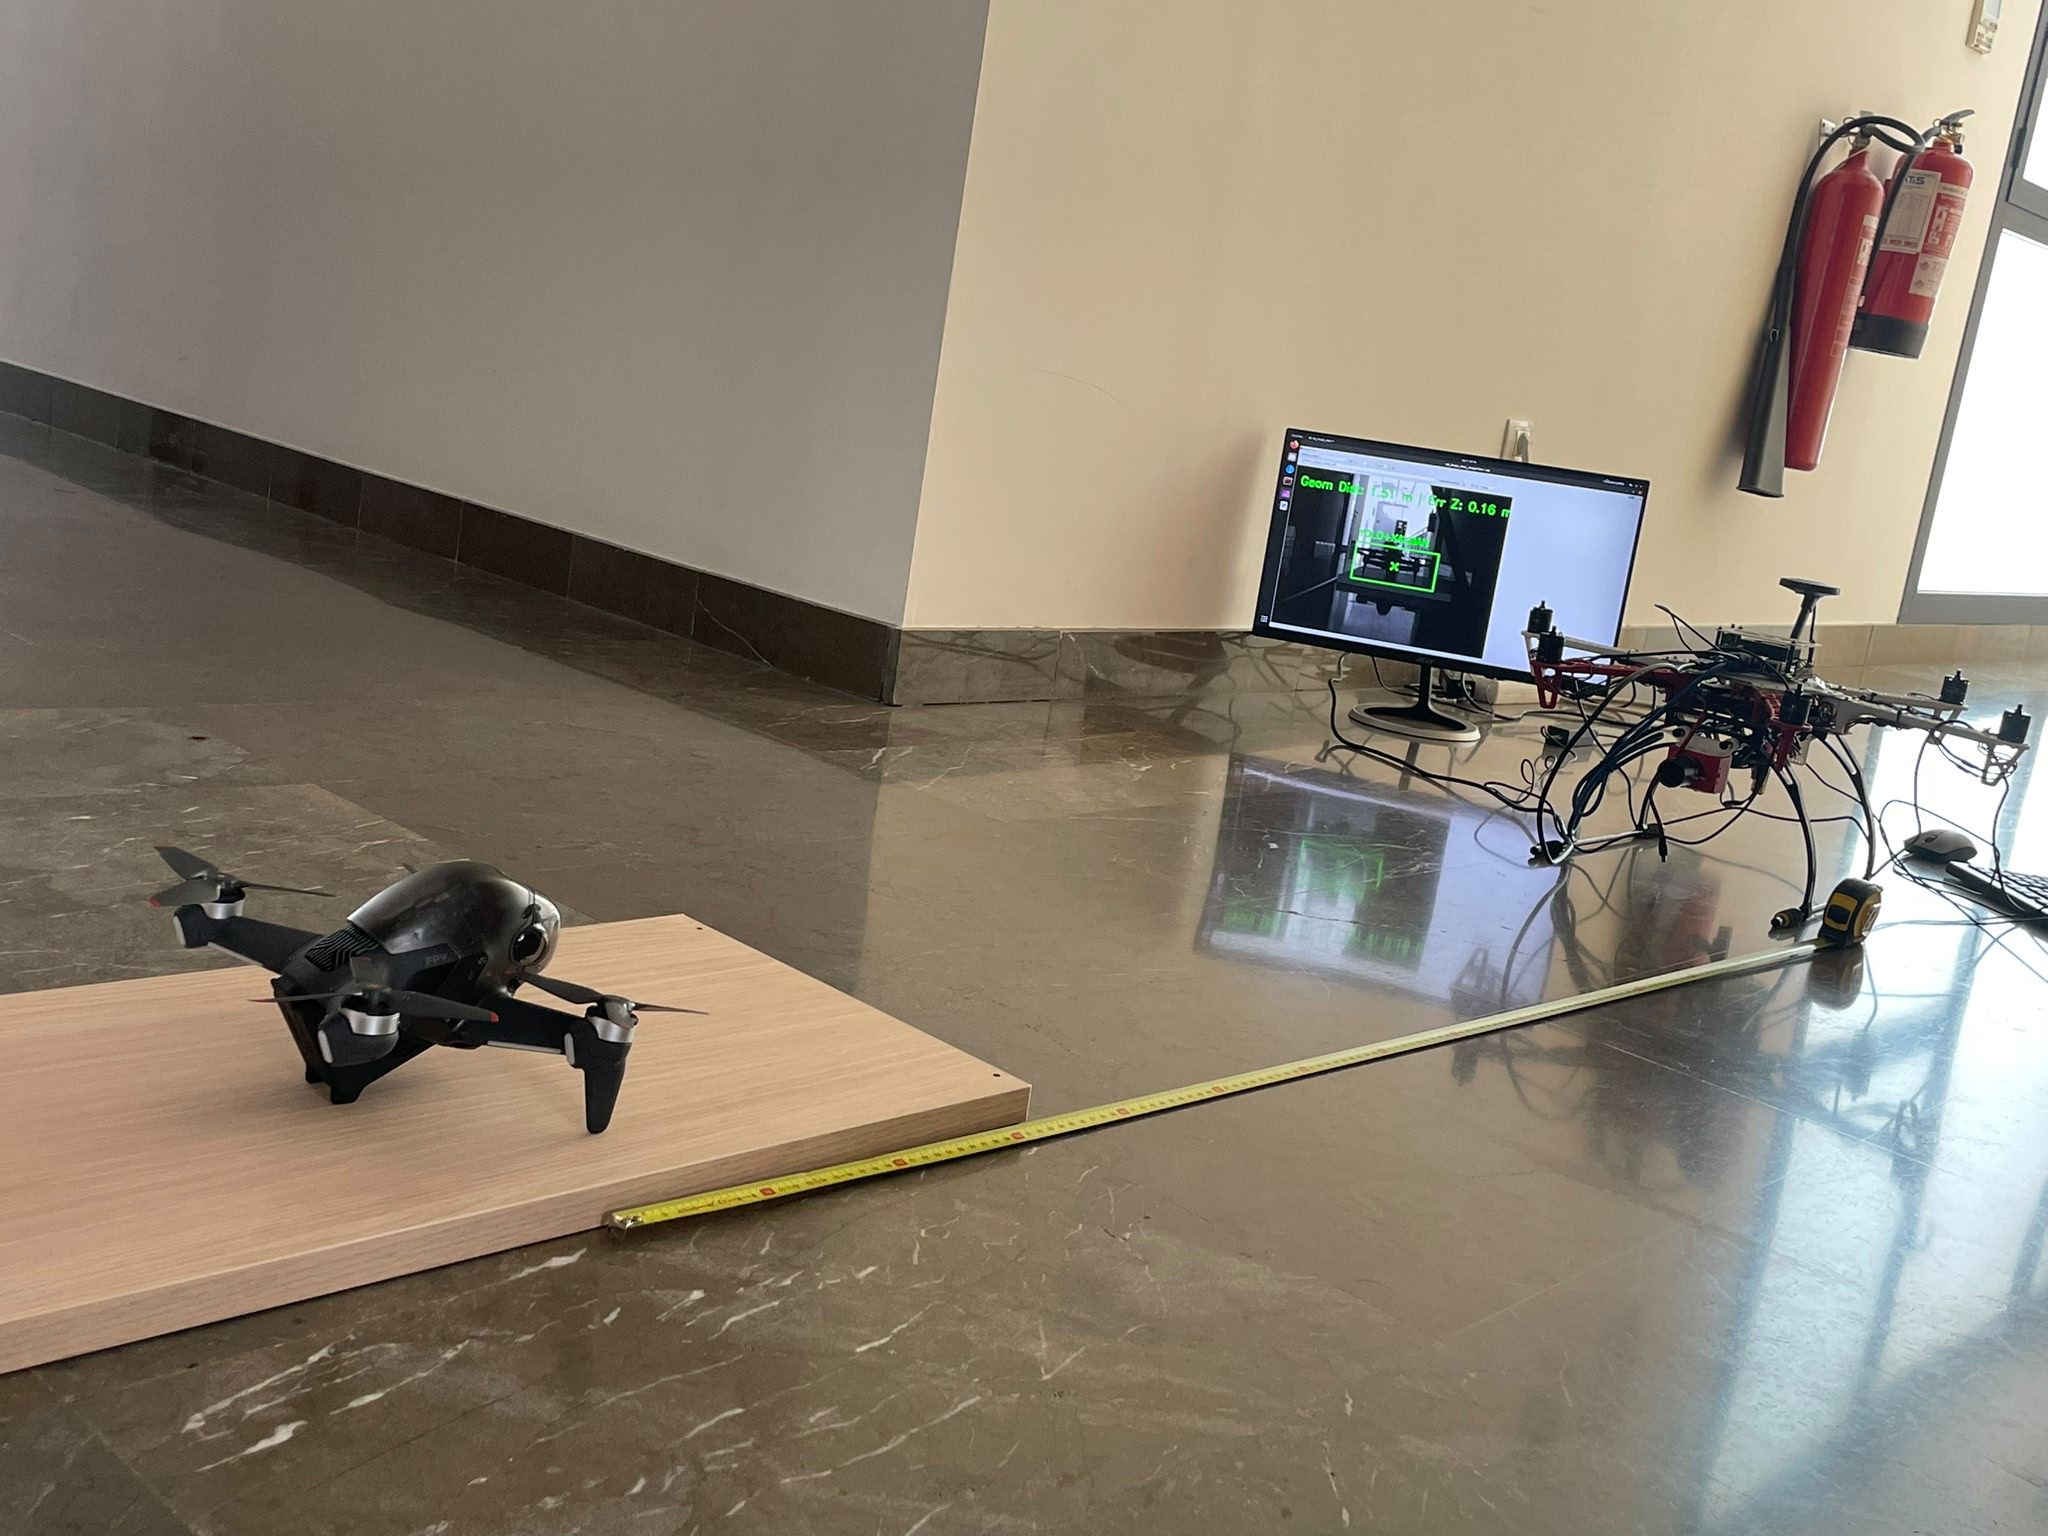
\includegraphics[width=0.82\textwidth]{imagenes/DronpruebaDist.jpeg}
\caption{Montaje utilizado para la prueba real de estimación de distancia. (Imagen de Elaboración Propia)}
\label{fig:dron-prueba-distancia}
\end{figure}

\vspace{0.3cm}

Las Figuras \ref{fig:dron-real-1m} y \ref{fig:dron-real-575cm} muestran dos ejemplos de la imagen observada por la cámara durante la prueba. En la primera se representa una distancia cercana de aproximadamente $1\,\mathrm{m}$, donde el dron ocupa una región grande de la imagen y la caja delimitadora dispone de más píxeles para estimar la anchura. En la segunda se muestra una distancia mucho mayor, cercana a $5.75\,\mathrm{m}$, donde el tamaño aparente del UAV se reduce de forma considerable y cualquier pequeña variación de la caja tiene más efecto sobre la estimación final.

\begin{figure}[H]
\centering
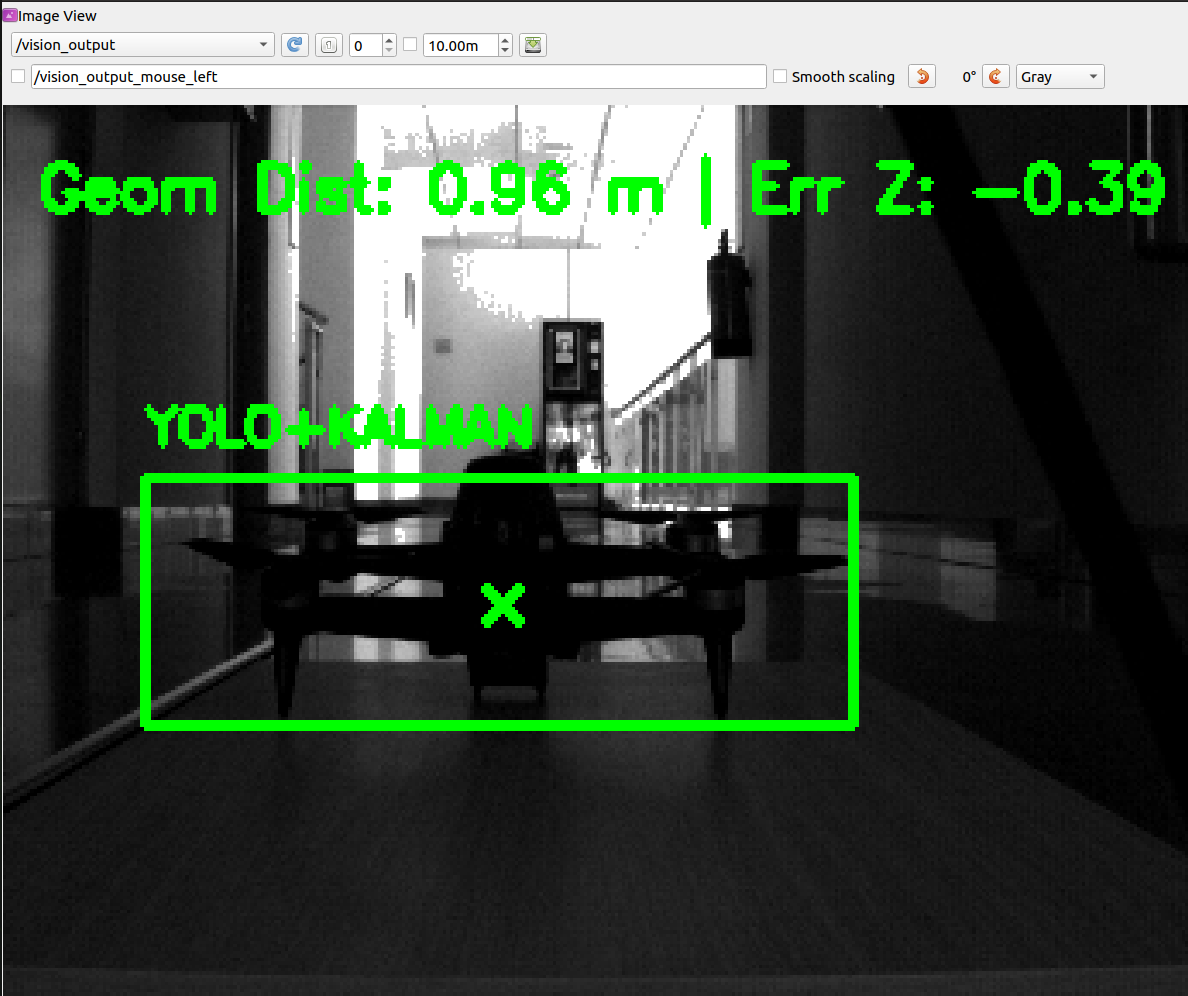
\includegraphics[width=0.9\textwidth]{imagenes/Dron1m_3.png}
\caption{Vista del UAV objetivo a una distancia aproximada de $1\,\mathrm{m}$. (Imagen de Elaboración Propia)}
\label{fig:dron-real-1m}
\end{figure}

\begin{figure}[H]
\centering
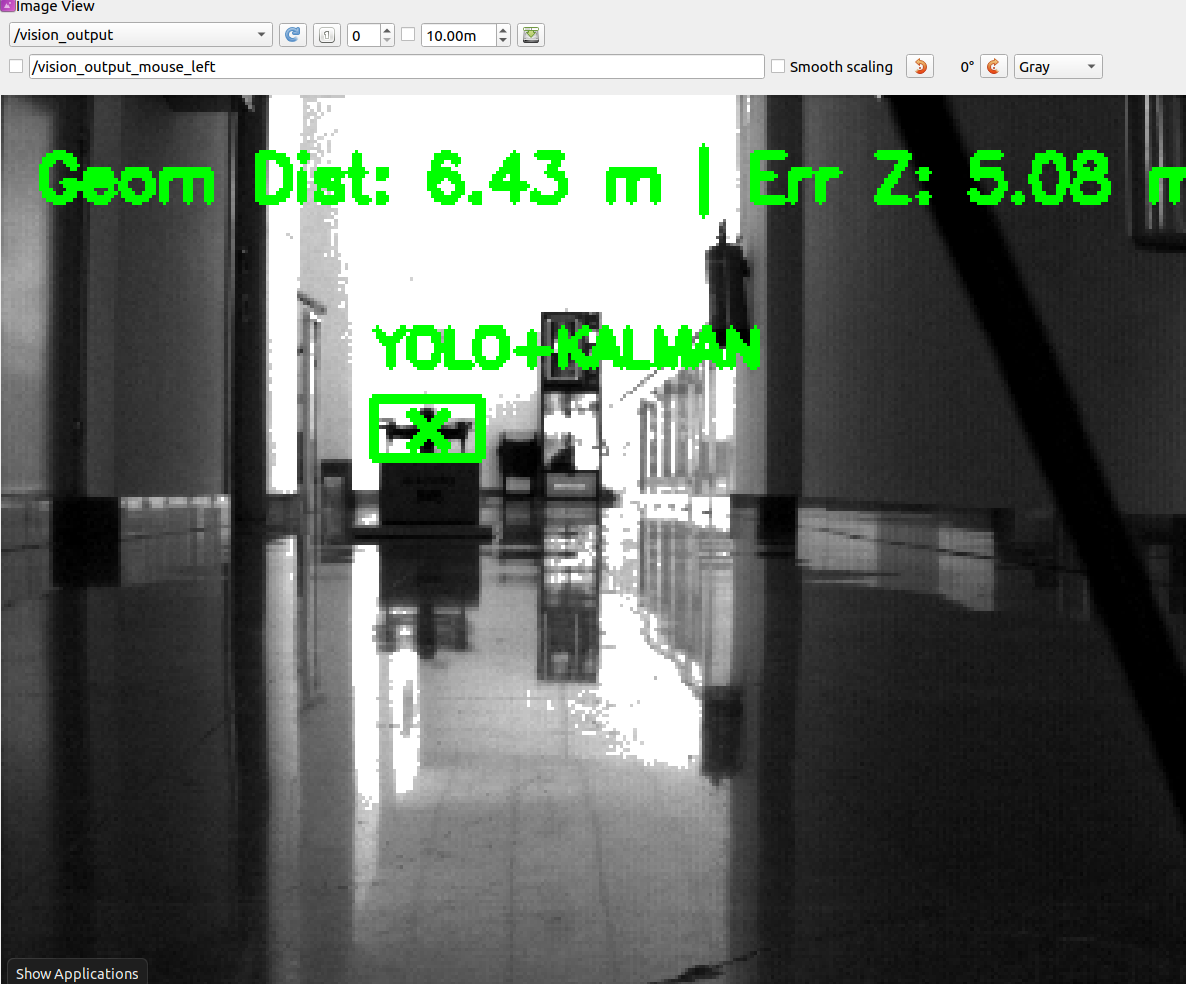
\includegraphics[width=0.9\textwidth]{imagenes/Dron575cm.png}
\caption{Vista del UAV objetivo a una distancia aproximada de $5.75\,\mathrm{m}$. (Imagen de Elaboración Propia)}
\label{fig:dron-real-575cm}
\end{figure}

\vspace{0.3cm}

A partir de las cinco repeticiones realizadas se generaron las gráficas de error de las Figuras \ref{fig:grafica-error-distancia-repeticiones} y \ref{fig:grafica-error-distancia-media}. En la primera se representa el error de estimación obtenido en cada una de las cinco pruebas, expresado en centímetros, frente a la distancia real en metros. En la segunda se muestra el error medio para cada distancia junto con la desviación típica, representada mediante una zona sombreada correspondiente a $\pm 1$ desviación típica. De este modo, la primera gráfica permite comparar las repeticiones individuales, mientras que la segunda resume la tendencia general y la variabilidad del modelo.

\begin{figure}[H]
\centering
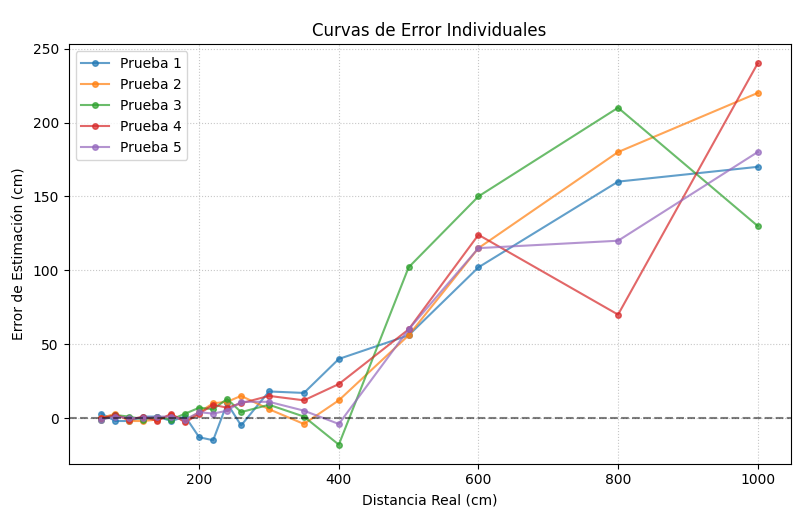
\includegraphics[width=1.0\textwidth]{imagenes/Esti_dist.png}
\caption{Errores de estimación de distancia obtenidos en las cinco pruebas realizadas con la cámara real y el UAV objetivo real. (Imagen de Elaboración Propia)}
\label{fig:grafica-error-distancia-repeticiones}
\end{figure}


\begin{figure}[H]
\centering
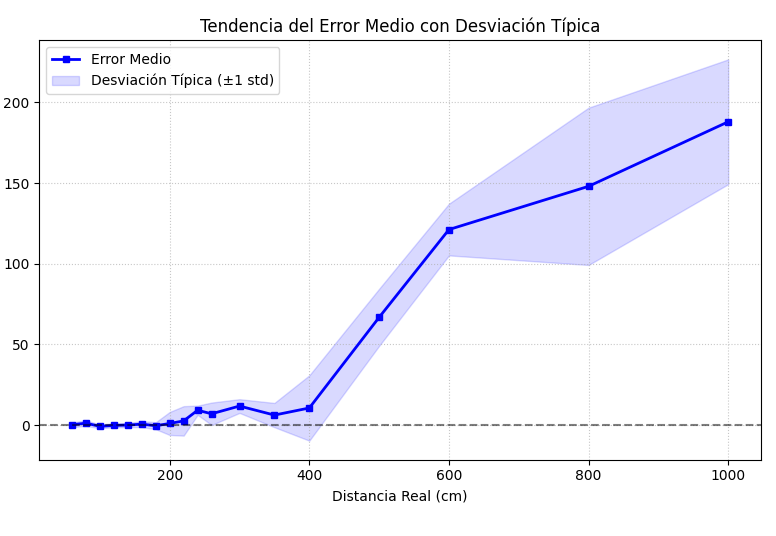
\includegraphics[width=1.0\textwidth]{imagenes/Esti_dist_der.png}
\caption{Error medio de estimación de distancia con la desviación típica sombreada para las cinco pruebas realizadas. (Imagen de Elaboración Propia)}
\label{fig:grafica-error-distancia-media}
\end{figure}

\vspace{0.2cm}

Las métricas globales obtenidas para el modelo de distancia se resumen en la Tabla \ref{tab:metricas-distancia-real}. El error medio absoluto fue de $33.68\,\mathrm{cm}$ y la desviación típica total alcanzó $58.48\,\mathrm{cm}$. Estos valores reflejan que la estimación mantiene una relación útil con la distancia real, pero también que existe una variabilidad apreciable entre repeticiones, especialmente cuando el objetivo ocupa pocos píxeles en la imagen.

\begin{table}[H]
\centering
\caption{Métricas globales del modelo de estimación de distancia con cámara real.}
\label{tab:metricas-distancia-real}
\begin{tabular}{lc}
\hline
\textbf{Métrica} & \textbf{Valor} \\
\hline
Error Medio Absoluto (MAE) & $33.68\,\mathrm{cm}$ \\
Desviación típica total & $58.48\,\mathrm{cm}$ \\
\hline
\end{tabular}
\end{table}

\vspace{0.2cm}

Los resultados muestran que, para distancias cortas y medias, el error se mantiene más acotado en comparación con las zonas de mayor separación. En la zona inicial de la gráfica aparecen desviaciones positivas y negativas de menor magnitud, lo que indica que el sistema puede sobreestimar o subestimar la distancia, pero sin perder una relación coherente entre el tamaño aparente del dron y la separación real. Este comportamiento es esperable, ya que a corta distancia la caja delimitadora ocupa más píxeles y la estimación basada en anchura es menos sensible a pequeñas variaciones de la detección.

\vspace{0.2cm}

A medida que aumenta la distancia, el error y la dispersión entre repeticiones crecen de forma más clara. En particular, a partir de aproximadamente $3.5\,\mathrm{m}$ se observa que la estimación comienza a degradarse ligeramente y aparecen diferencias más apreciables entre pruebas. Esto se debe a que el UAV aparece cada vez más pequeño en la imagen: una diferencia de pocos píxeles en la anchura de la caja representa una variación mayor en la distancia calculada. Además, a distancias largas influyen más la resolución de la cámara, la estabilidad de la detección, la orientación del dron y la calidad de la calibración. Por este motivo, la desviación típica sombreada en la gráfica resulta especialmente útil para interpretar la fiabilidad de la estimación en cada rango de distancia.

\vspace{0.2cm}

En conjunto, la prueba confirma que el sistema de estimación resulta útil para trabajar en rangos cercanos y medios, que son los más relevantes para iniciar y mantener un seguimiento visual seguro. No obstante, también evidencia que la precisión empieza a verse afectada a partir de unos $3.5\,\mathrm{m}$ y que la variabilidad aumenta cuando el objetivo se encuentra más alejado y ocupa pocos píxeles en la imagen. Por tanto, para pruebas reales de persecución conviene tener en cuenta esta degradación progresiva y utilizar la distancia estimada como una referencia de control dentro del rango en el que la detección se mantiene suficientemente estable.

\vspace{0.2cm}




\section{Análisis de Resultados}

Los resultados obtenidos permiten valorar el comportamiento general del sistema desde cinco puntos de vista: la detección visual, la optimización de inferencia, el control del UAV cazador, el seguimiento en simulación y la estimación de distancia con cámara real. Esta lectura conjunta es importante, ya que el buen funcionamiento del sistema no depende de un único elemento, sino de la coordinación entre percepción y control.

\vspace{0.2cm}

La Tabla \ref{tab:analisis-cumplimiento-resultados} resume el grado de cumplimiento de las pruebas realizadas. Se considera que un punto está cumplido cuando el resultado responde al objetivo principal de la prueba, y cumplido parcialmente cuando el sistema funciona, pero todavía muestra alguna limitación relevante.

\begin{table}[H]
\centering
\caption{Resumen del grado de cumplimiento de las pruebas realizadas.}
\label{tab:analisis-cumplimiento-resultados}
\scriptsize
\setlength{\tabcolsep}{3pt}
\begin{tabular}{p{0.25\textwidth}p{0.18\textwidth}p{0.47\textwidth}}
\hline
\textbf{Punto evaluado} & \textbf{Resultado} & \textbf{Justificación} \\
\hline
Selección del detector visual & Cumplido & YOLOv8n ofrece un buen equilibrio entre precisión, tamaño y velocidad, con \textit{mAP50} de 0.992507, \textit{mAP50-95} de 0.733692 y 2.660333 ms de inferencia. \\
Optimización con TensorRT & Cumplido & La conversión a \texttt{.engine} FP16 reduce el tiempo total de 22.53 ms a 11.74 ms y eleva los FPS teóricos de 44.4 a 85.2, dejando margen suficiente para una cámara de 30 FPS. \\
Control de \textit{yaw} & Cumplido & El error horizontal se corrige con rapidez, con un tiempo de establecimiento aproximado de $0.65\,\mathrm{s}$. \\
Control de altura & Cumplido & El error vertical se reduce de forma estable, con un tiempo de establecimiento aproximado de $1.25\,\mathrm{s}$. \\
Control de distancia & Cumplido parcialmente & Mantiene una separación segura, aunque responde más lento que los otros ejes, con $T_s \approx 6\,\mathrm{s}$. \\
Seguimiento visual en simulación & Cumplido & En las trayectorias evaluadas no se perdió el objetivo, con TLR del $0.00\%$ y detección YOLO igual o superior al $99.74\%$. \\
Seguimiento en zigzag & Cumplido parcialmente & El objetivo se mantiene visible durante toda la prueba, aunque la distancia presenta más error, con RMSE de $1.255\,\mathrm{m}$. \\
Trayectoria circular ondulada & Cumplido & Se obtiene seguimiento estable, con EPE medio de 0.0513 y RMSE de distancia de $0.2200\,\mathrm{m}$. \\
Ruta final por \textit{waypoints} & Cumplido & El sistema mantiene un TLR nulo, detección YOLO del $99.98\%$ y EPE medio total de 0.0221. \\
Estimación de distancia con cámara real & Cumplido parcialmente & La estimación es útil en distancias cortas y medias, aunque a partir de unos $3.5\,\mathrm{m}$ empieza a perder estabilidad; el MAE fue de $33.68\,\mathrm{cm}$. \\
Seguimiento real completo & Pendiente & No se valida todavía una persecución real completa con ambos UAV en vuelo, sino una primera prueba real de estimación de distancia. \\
\hline
\end{tabular}
\end{table}

\vspace{0.3cm}

En percepción, el objetivo principal se considera cumplido. YOLOv8n fue seleccionado porque combina una precisión alta con un tiempo de inferencia bajo, lo que facilita su uso dentro del lazo de control. Además, la conversión a TensorRT redujo de forma notable la latencia del detector, pasando de 22.53 ms a 11.74 ms por frame, lo que incrementa el margen temporal disponible para el resto de procesos del sistema. En las pruebas de seguimiento, el detector mantuvo porcentajes de detección muy altos y no se produjo pérdida completa del UAV objetivo en simulación.

\vspace{0.2cm}

En cuanto al control, los resultados son claros en los ejes de \textit{yaw} y altura. Ambos controladores corrigen el error de forma rápida y estable, permitiendo que el objetivo vuelva al centro de la imagen. El control de distancia también cumple su función principal, ya que mantiene una separación segura, aunque su respuesta es más lenta y muestra más dificultad en trayectorias como el zigzag.

\vspace{0.2cm}

Las pruebas de seguimiento en simulación muestran un comportamiento global positivo. El sistema fue capaz de seguir al UAV objetivo en trayectorias con cambios laterales, variaciones de altura y rutas por \textit{waypoints}. Aunque el eje de distancia sigue siendo el más exigente, la referencia visual se mantuvo durante las pruebas y el seguimiento no se interrumpió.

\vspace{0.2cm}

En las pruebas reales, la estimación de distancia funcionó de forma coherente en rangos cercanos y medios. Sin embargo, a partir de aproximadamente $3.5\,\mathrm{m}$ el objetivo ocupa menos píxeles en la imagen y la estimación empieza a ser menos estable. Por ello, en ese rango conviene que el control actúe de forma más conservadora y se apoye en la continuidad de la detección visual.

\vspace{0.3cm}

En conjunto, los objetivos principales del capítulo quedan cubiertos: se selecciona un detector adecuado, se optimiza su ejecución mediante TensorRT, se valida el centrado visual, se comprueba el seguimiento en simulación y se realiza una primera prueba real de distancia. Las principales líneas de mejora se centran en ajustar el control longitudinal, mejorar la estimación de profundidad a distancias mayores y avanzar hacia una validación real completa con ambos UAV en vuelo.
